\documentclass[notes,10pt, aspectratio=169]{beamer}

\usepackage{pgfpages}
% These slides also contain speaker notes. You can print just the slides,
% just the notes, or both, depending on the setting below. Comment out the want
% you want.
\setbeameroption{hide notes} % Only slide
%\setbeameroption{show only notes} % Only notes
%\setbeameroption{show notes on second screen=right} % Both
\usepackage{wrapfig}

\usepackage{helvet}
\usepackage[default]{lato}
\usepackage{array}
\usepackage{eurosym}
\usepackage{setspace}
\usepackage{animate}
\usepackage{multicol}
\usepackage{breqn}
\usepackage{subcaption}
\usepackage{caption}
\captionsetup{font=scriptsize, justification=raggedright,singlelinecheck=false}
\usepackage[export]{adjustbox}
\usepackage[scale=2]{ccicons}
\usepackage{tikz}
\newenvironment{wideitemize}{\itemize\addtolength{\itemsep}{10pt}}{\enditemize}
\usepackage{natbib}

\usepackage{tikz}
\usepackage{verbatim}
\setbeamertemplate{note page}{\pagecolor{yellow!5}\insertnote}
\usepackage{amsmath}
\usepackage{bm}
%\usepackage{mathpazo}
\usepackage{hyperref}
\usepackage{lipsum}
\usepackage{multimedia}
\usepackage{multirow}
\usepackage{graphicx}
\usepackage{dcolumn}
\usepackage{bbm}
\newcolumntype{d}[0]{D{.}{.}{5}}

\usepackage{changepage}
\usepackage{appendixnumberbeamer}
% \newcommand{\beginbackup}{
%   \newcounter{framenumbervorappendix}
%   \setcounter{framenumbervorappendix}{\value{framenumber}}
%   \setbeamertemplate{footline}
%   {
%      \leavevmode%
%      \hline
%      box{%
%       \begin{beamercolorbox}[wd=\paperwidth,ht=2.25ex,dp=1ex,right]{footlinecolor}%
% %         \insertframenumber  \hspace*{2ex} 
%       \end{beamercolorbox}}%
%      \vskip0pt%
%   }
%  }
\useinnertheme[shadow]{rounded}
\setbeamercolor{block title example}{fg=black,bg=orange!50!white}
\setbeamercolor{block body example}{fg=black, bg=orange!30!white}
\setbeamercolor{block title}{use=structure,fg=structure.fg,bg=structure.fg!20!bg}
\setbeamercolor{block body}{parent=normal text,use=block title,bg=block title.bg!50!bg}

 \setbeamertemplate{footline}{
    \hbox{%
    \begin{beamercolorbox}[wd=\paperwidth,ht=3ex,dp=1.5ex,leftskip=2ex,rightskip=2ex]{page footer}%
        %\usebeamerfont{title in head/foot}%
        %\insertshorttitle \hfill
        %\insertsection \hfill
        %\tableofcontents[currentsection] \hfill
        \insertsectionnavigationhorizontal{0.7\paperwidth}{}{} \hfill 
        \insertframenumber{} / \inserttotalframenumber
    \end{beamercolorbox}}%
}
\newcommand{\backupend}{
   \addtocounter{framenumbervorappendix}{-\value{framenumber}}
   \addtocounter{framenumber}{\value{framenumbervorappendix}} 
}


\usepackage{graphicx}
\usepackage[space]{grffile}
\usepackage{booktabs}

% These are my colors -- there are many like them, but these ones are mine.
\definecolor{blue}{RGB}{0,114,178}
\definecolor{red}{RGB}{213,94,0}
\definecolor{yellow}{RGB}{240,228,66}
\definecolor{green}{RGB}{0,158,115}

\setbeamercolor{section in head/foot}{fg=blue}


\hypersetup{
  colorlinks=false,
  linkbordercolor = {white},
  linkcolor = {blue}
}


%% I use a beige off white for my background
\definecolor{MyBackground}{RGB}{255,253,218}

%% Uncomment this if you want to change the background color to something else
%\setbeamercolor{background canvas}{bg=MyBackground}

%% Change the bg color to adjust your transition slide background color!
\newenvironment{transitionframe}{
  \setbeamercolor{background canvas}{bg=yellow}
  \begin{frame}}{
    \end{frame}
}

\setbeamercolor{frametitle}{fg=blue}
\setbeamercolor{title}{fg=black}
%\setbeamertemplate{footline}[frame number]
\setbeamertemplate{navigation symbols}{} 
\setbeamertemplate{itemize items}{-}
\setbeamercolor{itemize item}{fg=blue}
\setbeamercolor{itemize subitem}{fg=blue}
\setbeamercolor{enumerate item}{fg=blue}
\setbeamercolor{enumerate subitem}{fg=blue}
\setbeamercolor{button}{bg=white,fg=blue,}



% If you like road maps, rather than having clutter at the top, have a roadmap show up at the end of each section 
% (and after your introduction)
% Uncomment this is if you want the roadmap!
% \AtBeginSection[]
% {
%    \begin{frame}
%        \frametitle{Roadmap of Talk}
%        \tableofcontents[currentsection]
%    \end{frame}
% }

\useinnertheme[shadow]{rounded}
\setbeamercolor{block title example}{fg=black,bg=orange!50!white}
\setbeamercolor{block body example}{fg=black, bg=orange!30!white}
\setbeamercolor{block title}{use=structure,fg=structure.fg,bg=structure.fg!20!bg}
\setbeamercolor{block body}{parent=normal text,use=block title,bg=block title.bg!50!bg}


\setbeamercolor{section in toc}{fg=blue}
\setbeamercolor{subsection in toc}{fg=red}
%\setbeamersize{text margin left=1em,text margin right=1em} 
\setbeamersize{text margin left=0.7cm,text margin right=0.7cm} 


\title[]{\textcolor{blue}{Lecture 5:\\Multivariate Linear Regression}}
\author{25117 - Econometrics}
\institute[shortinst]{Universitat Pompeu Fabra}

\date{October 16th, 2024}

\begin{document}



% Title Slide

\begin{frame}[plain]
\maketitle
\end{frame}

\section{Introduction}

\begin{frame}{What we learned in the last lesson}
\begin{itemize}
    \item Hypothesis testing for regression coefficients is analogous to hypothesis testing for the population mean: Use the t-statistic to calculate the p-values and either accept or reject the null hypothesis. Like a confidence interval for the population mean, a 95\% confidence interval for a regression coefficient is computed as the estimator $\pm$1.96 standard errors.\\[1em]
    \item When X is binary, the regression model can be used to estimate and test hypotheses about the difference between the population means of the “X = 0” group and the “X = 1” group.\\[1em]
    \item In general, the error $u_i$ is heteroskedastic; that is, the variance of $u_i$ at a given value of $X_i$, $var(u_i\mid X_i=x)$, depends on $x$. A special case is when the error is homoskedastic; that is, when $var(u_i\mid X_i=x)$ is constant. \\[1em]Homoskedasticity-only standard errors do not produce valid statistical inferences when the errors are heteroskedastic, but heteroskedasticity-robust standard errors do.\\[1em]
\end{itemize}
\end{frame}

\begin{frame}{What we learned in the last lesson}
\begin{itemize}
    \item If the three least squares assumption hold and if the regression errors are homoskedastic, then, as a result of the Gauss–Markov theorem, the OLS estimator is BLUE.\\[1em]
    \item If the three least squares assumptions hold, if the regression errors are homoskedastic, and if the regression errors are normally distributed, then the OLS t-statistic computed using homoskedasticity-only standard errors has a Student t distribution when the null hypothesis is true. The difference between the Student t distribution and the normal distribution is negligible if the sample size is moderate or large.\\[1em]
\end{itemize}
\end{frame}

\begin{frame}{Omitted Variable Bias (OVB)}
\begin{itemize}
    \item If $\beta_1$ is a causal effect, the first assumption of the Gauss-Markov Theorem must hold : $\mathbb{E}(u_i\mid X_i)=0$ for all $i$
    \item Remember that $\hat{\beta}_1= \beta_1+\frac{cov(X,u)}{var(X)}$ and $\hat{\beta}_1$ will be unbiased only if $\mathbb{E}(\frac{cov(X,u)}{var(X)})=0$
    \item \textbf{Example:}
    \begin{itemize}
      \item Private university graduates tend to have higher wages than public university graduates. Does that mean that private university education ($X_1$) yields higher wages ($Y$)?
      \item Maybe, but not necessarily --- Private university graduates are \textit{selected} by those institutions
      \item They differ in a number of ways from public university graduates: they have on average better test scores in highschool, they come from wealthier families, etc.
      \item All these relevant but unobserved variables may be omitted, and, if not accounted for, may bias the estimation of $\beta_1$
      \item In comparing wages from private and public university graduates, how to \textit{identify} the causal effect of education ($X_1$) and differentiate it from the effect of, say, advantageous social background?
      \item We want to make apple-to-apple comparisons...
    \end{itemize}
    \end{itemize}
\end{frame}



\begin{frame}{Omitted Variable Bias (OVB)}
The bias in the OLS estimator that occurs as a result of an omitted factor, or variable, is called omitted variable bias. For omitted variable bias to occur, the omitted variable $Z$ must satisfy two conditions:
\begin{enumerate}
    \item $Z$ is a determinant of $Y$ (i.e. $Z$ is part of $u$); and
    \item $Z$ is correlated with the regressor $X$ (i.e., $corr(Z,X)\neq 0)$
\end{enumerate}

\begin{center}
\begin{figure}
    \resizebox{.6\linewidth}{!}{%



\tikzset{every picture/.style={line width=0.75pt}} %set default line width to 0.75pt        

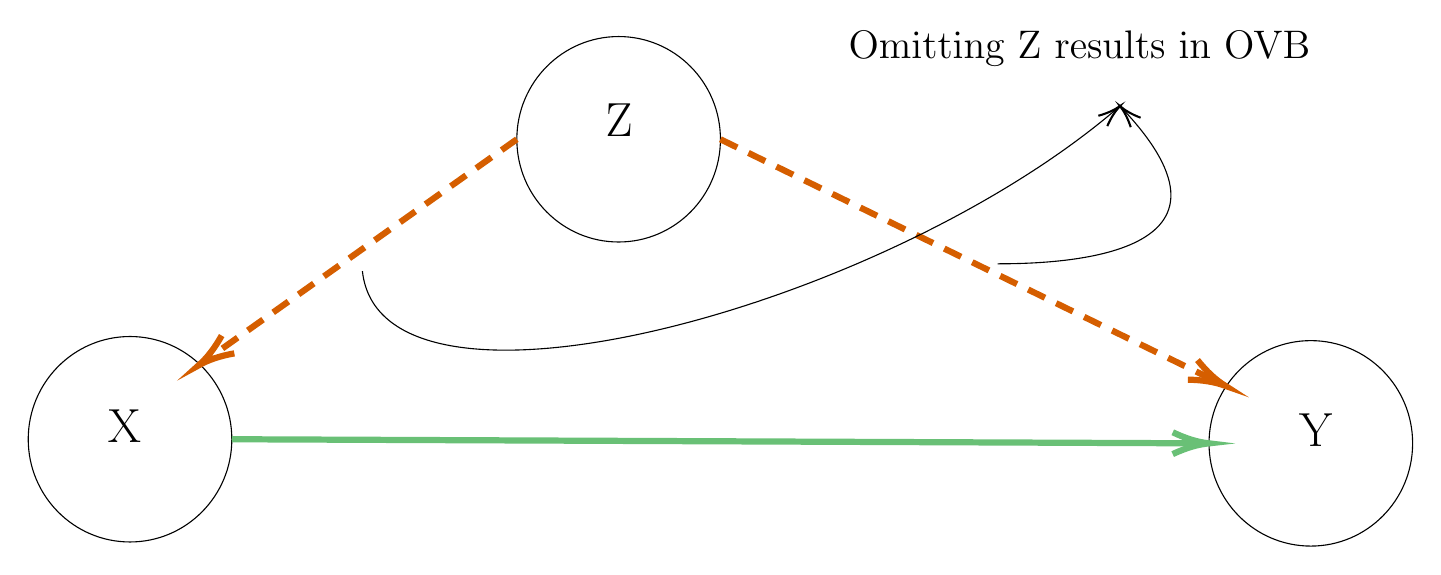
\begin{tikzpicture}[x=0.75pt,y=0.75pt,yscale=-1,xscale=1]
%uncomment if require: \path (0,285); %set diagram left start at 0, and has height of 285

%Shape: Ellipse [id:dp36615011120920427] 
\draw   (254.41,66.5) .. controls (254.41,39.16) and (276.37,17) .. (303.46,17) .. controls (330.54,17) and (352.5,39.16) .. (352.5,66.5) .. controls (352.5,93.83) and (330.54,115.99) .. (303.46,115.99) .. controls (276.37,115.99) and (254.41,93.83) .. (254.41,66.5) -- cycle ;
%Shape: Ellipse [id:dp34906029723118115] 
\draw   (19,211.02) .. controls (19,183.69) and (40.96,161.53) .. (68.04,161.53) .. controls (95.13,161.53) and (117.09,183.69) .. (117.09,211.02) .. controls (117.09,238.36) and (95.13,260.52) .. (68.04,260.52) .. controls (40.96,260.52) and (19,238.36) .. (19,211.02) -- cycle ;
%Shape: Ellipse [id:dp6974919182309072] 
\draw   (587.91,213) .. controls (587.91,185.67) and (609.87,163.51) .. (636.96,163.51) .. controls (664.04,163.51) and (686,185.67) .. (686,213) .. controls (686,240.34) and (664.04,262.5) .. (636.96,262.5) .. controls (609.87,262.5) and (587.91,240.34) .. (587.91,213) -- cycle ;
%Straight Lines [id:da04124970397057681] 
\draw [color={rgb, 255:red, 126; green, 211; blue, 33 }  ,draw opacity=1 ][line width=2.25]    (117.09,211.02) -- (583.91,212.99) ;
\draw [shift={(587.91,213)}, rotate = 180.24] [color={rgb, 255:red, 126; green, 211; blue, 33 }  ,draw opacity=1 ][line width=2.25]    (17.49,-5.26) .. controls (11.12,-2.23) and (5.29,-0.48) .. (0,0) .. controls (5.29,0.48) and (11.12,2.23) .. (17.49,5.26)   ;
%Straight Lines [id:da035209354566531736] 
\draw [color={rgb, 255:red, 255; green, 0; blue, 0 }  ,draw opacity=1 ][line width=2.25]  [dash pattern={on 6.75pt off 4.5pt}]  (254.41,66.5) -- (104.26,173.18) ;
\draw [shift={(101,175.5)}, rotate = 324.6] [color={rgb, 255:red, 255; green, 0; blue, 0 }  ,draw opacity=1 ][line width=2.25]    (17.49,-5.26) .. controls (11.12,-2.23) and (5.29,-0.48) .. (0,0) .. controls (5.29,0.48) and (11.12,2.23) .. (17.49,5.26)   ;
%Straight Lines [id:da19389419961485554] 
\draw [color={rgb, 255:red, 255; green, 0; blue, 0 }  ,draw opacity=1 ][line width=2.25]  [dash pattern={on 6.75pt off 4.5pt}]  (352.5,66.5) -- (592.16,183.53) ;
\draw [shift={(595.76,185.29)}, rotate = 206.03] [color={rgb, 255:red, 255; green, 0; blue, 0 }  ,draw opacity=1 ][line width=2.25]    (17.49,-5.26) .. controls (11.12,-2.23) and (5.29,-0.48) .. (0,0) .. controls (5.29,0.48) and (11.12,2.23) .. (17.49,5.26)   ;
%Curve Lines [id:da92152652585756] 
\draw    (486,126.5) .. controls (518.84,126.5) and (613.05,122.54) .. (546.02,51.57) ;
\draw [shift={(545,50.5)}, rotate = 46.22] [color={rgb, 255:red, 0; green, 0; blue, 0 }  ][line width=0.75]    (10.93,-3.29) .. controls (6.95,-1.4) and (3.31,-0.3) .. (0,0) .. controls (3.31,0.3) and (6.95,1.4) .. (10.93,3.29)   ;
%Curve Lines [id:da6333756929191379] 
\draw    (180,130) .. controls (189,213) and (432,148.5) .. (545,50.5) ;
\draw [shift={(545,50.5)}, rotate = 139.07] [color={rgb, 255:red, 0; green, 0; blue, 0 }  ][line width=0.75]    (10.93,-3.29) .. controls (6.95,-1.4) and (3.31,-0.3) .. (0,0) .. controls (3.31,0.3) and (6.95,1.4) .. (10.93,3.29)   ;

% Text Node
\draw (56.08,195.51) node [anchor=north west][inner sep=0.75pt]   [align=left] {{\LARGE X}};
% Text Node
\draw (295.97,47.97) node [anchor=north west][inner sep=0.75pt]   [align=left] {{\LARGE Z}};
% Text Node
\draw (630.08,197.51) node [anchor=north west][inner sep=0.75pt]   [align=left] {{\LARGE Y}};
% Text Node
\draw (413,13) node [anchor=north west][inner sep=0.75pt]  [font=\Large] [align=left] {Omitting Z results in OVB};


\end{tikzpicture}

}
\end{figure}
\end{center}

Both conditions must hold for the omission of $Z$ to result in omitted variable bias.

\end{frame}




\begin{frame}{Omitted Variable Bias (OVB)}
The bias in the OLS estimator that occurs as a result of an omitted factor, or variable, is called omitted variable bias. For omitted variable bias to occur, the omitted variable $Z$ must satisfy two conditions:
\begin{enumerate}
    \item $Z$ is a determinant of $Y$ (i.e. $Z$ is part of $u$); and
    \item $Z$ is correlated with the regressor $X$ (i.e., $corr(Z,X)\neq 0)$
\end{enumerate}

\begin{center}
\begin{figure}
    \resizebox{.6\linewidth}{!}{%


\tikzset{every picture/.style={line width=0.75pt}} %set default line width to 0.75pt        

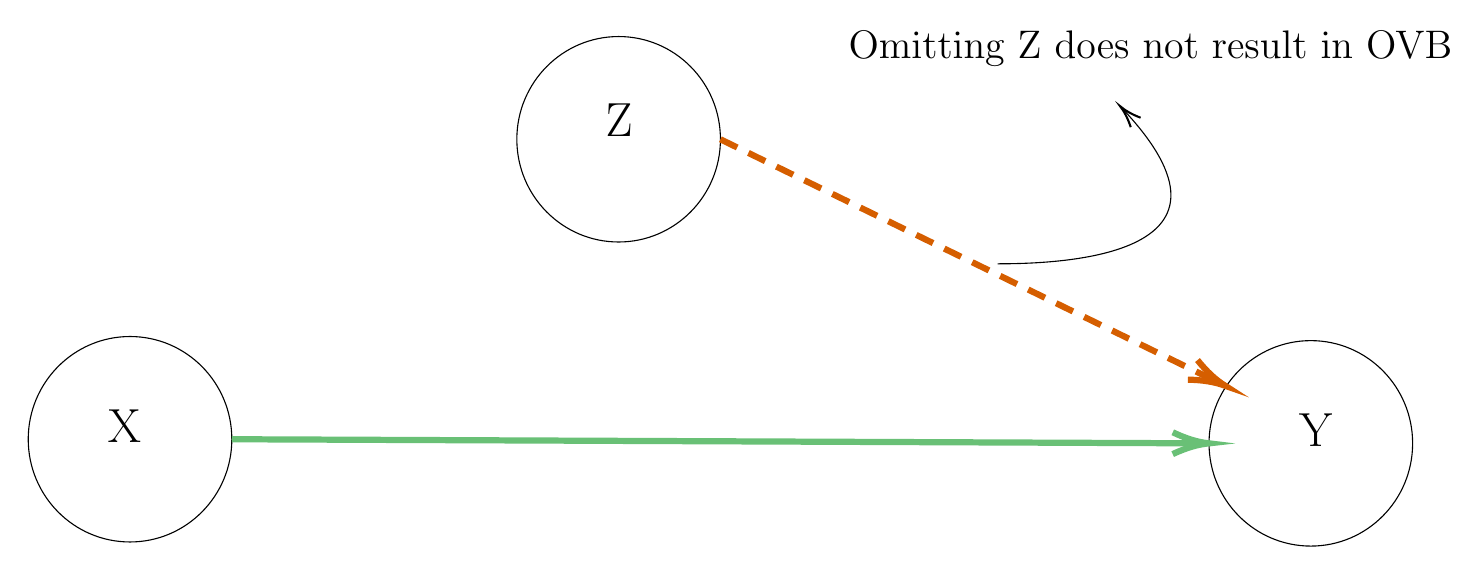
\begin{tikzpicture}[x=0.75pt,y=0.75pt,yscale=-1,xscale=1]
%uncomment if require: \path (0,285); %set diagram left start at 0, and has height of 285

%Shape: Ellipse [id:dp36615011120920427] 
\draw   (254.41,66.5) .. controls (254.41,39.16) and (276.37,17) .. (303.46,17) .. controls (330.54,17) and (352.5,39.16) .. (352.5,66.5) .. controls (352.5,93.83) and (330.54,115.99) .. (303.46,115.99) .. controls (276.37,115.99) and (254.41,93.83) .. (254.41,66.5) -- cycle ;
%Shape: Ellipse [id:dp34906029723118115] 
\draw   (19,211.02) .. controls (19,183.69) and (40.96,161.53) .. (68.04,161.53) .. controls (95.13,161.53) and (117.09,183.69) .. (117.09,211.02) .. controls (117.09,238.36) and (95.13,260.52) .. (68.04,260.52) .. controls (40.96,260.52) and (19,238.36) .. (19,211.02) -- cycle ;
%Shape: Ellipse [id:dp6974919182309072] 
\draw   (587.91,213) .. controls (587.91,185.67) and (609.87,163.51) .. (636.96,163.51) .. controls (664.04,163.51) and (686,185.67) .. (686,213) .. controls (686,240.34) and (664.04,262.5) .. (636.96,262.5) .. controls (609.87,262.5) and (587.91,240.34) .. (587.91,213) -- cycle ;
%Straight Lines [id:da04124970397057681] 
\draw [color={rgb, 255:red, 126; green, 211; blue, 33 }  ,draw opacity=1 ][line width=2.25]    (117.09,211.02) -- (583.91,212.99) ;
\draw [shift={(587.91,213)}, rotate = 180.24] [color={rgb, 255:red, 126; green, 211; blue, 33 }  ,draw opacity=1 ][line width=2.25]    (17.49,-5.26) .. controls (11.12,-2.23) and (5.29,-0.48) .. (0,0) .. controls (5.29,0.48) and (11.12,2.23) .. (17.49,5.26)   ;
%Straight Lines [id:da19389419961485554] 
\draw [color={rgb, 255:red, 255; green, 0; blue, 0 }  ,draw opacity=1 ][line width=2.25]  [dash pattern={on 6.75pt off 4.5pt}]  (352.5,66.5) -- (592.16,183.53) ;
\draw [shift={(595.76,185.29)}, rotate = 206.03] [color={rgb, 255:red, 255; green, 0; blue, 0 }  ,draw opacity=1 ][line width=2.25]    (17.49,-5.26) .. controls (11.12,-2.23) and (5.29,-0.48) .. (0,0) .. controls (5.29,0.48) and (11.12,2.23) .. (17.49,5.26)   ;
%Curve Lines [id:da92152652585756] 
\draw    (486,126.5) .. controls (518.84,126.5) and (613.05,122.54) .. (546.02,51.57) ;
\draw [shift={(545,50.5)}, rotate = 46.22] [color={rgb, 255:red, 0; green, 0; blue, 0 }  ][line width=0.75]    (10.93,-3.29) .. controls (6.95,-1.4) and (3.31,-0.3) .. (0,0) .. controls (3.31,0.3) and (6.95,1.4) .. (10.93,3.29)   ;

% Text Node
\draw (56.08,195.51) node [anchor=north west][inner sep=0.75pt]   [align=left] {{\LARGE X}};
% Text Node
\draw (295.97,47.97) node [anchor=north west][inner sep=0.75pt]   [align=left] {{\LARGE Z}};
% Text Node
\draw (630.08,197.51) node [anchor=north west][inner sep=0.75pt]   [align=left] {{\LARGE Y}};
% Text Node
\draw (413,13) node [anchor=north west][inner sep=0.75pt]  [font=\Large] [align=left] {Omitting Z does not result in OVB};


\end{tikzpicture}
}
\end{figure}
\end{center}

Both conditions must hold for the omission of $Z$ to result in omitted variable bias.

\end{frame}



\begin{frame}{Omitted Variable Bias (OVB)}
The bias in the OLS estimator that occurs as a result of an omitted factor, or variable, is called omitted variable bias. For omitted variable bias to occur, the omitted variable $Z$ must satisfy two conditions:
\begin{enumerate}
    \item $Z$ is a determinant of $Y$ (i.e. $Z$ is part of $u$); and
    \item $Z$ is correlated with the regressor $X$ (i.e., $corr(Z,X)\neq 0)$
\end{enumerate}

\begin{center}
\begin{figure}
    \resizebox{.6\linewidth}{!}{%


\tikzset{every picture/.style={line width=0.75pt}} %set default line width to 0.75pt        

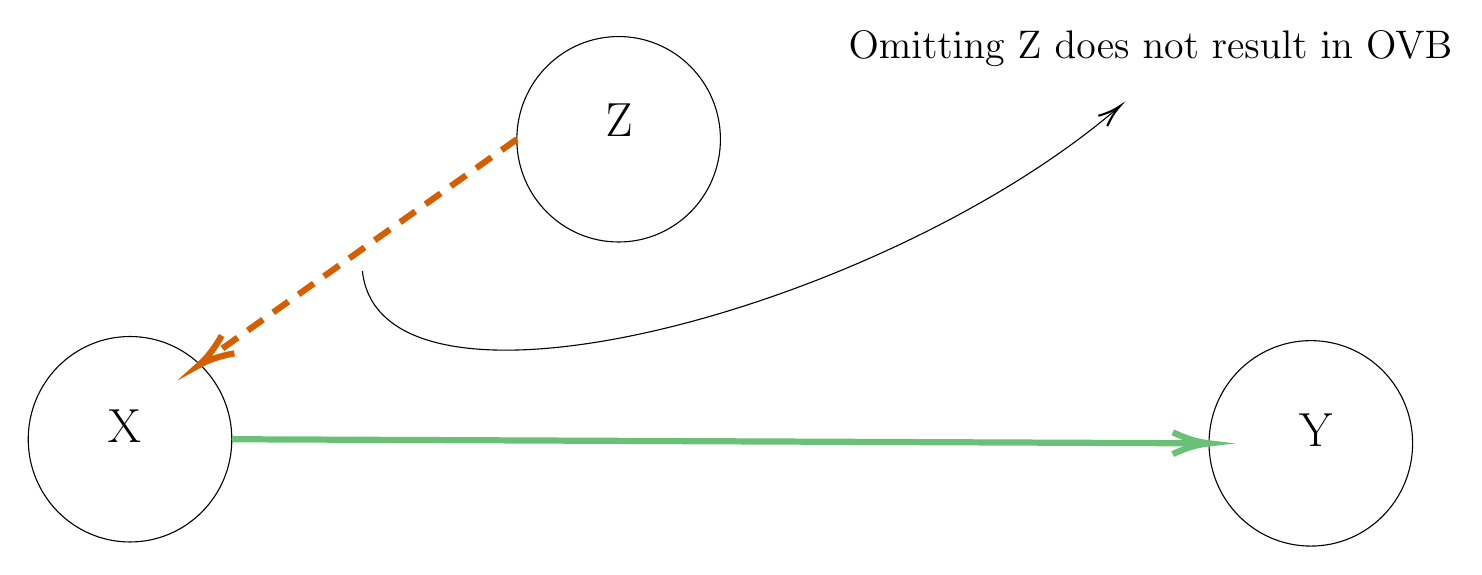
\begin{tikzpicture}[x=0.75pt,y=0.75pt,yscale=-1,xscale=1]
%uncomment if require: \path (0,285); %set diagram left start at 0, and has height of 285

%Shape: Ellipse [id:dp36615011120920427] 
\draw   (254.41,66.5) .. controls (254.41,39.16) and (276.37,17) .. (303.46,17) .. controls (330.54,17) and (352.5,39.16) .. (352.5,66.5) .. controls (352.5,93.83) and (330.54,115.99) .. (303.46,115.99) .. controls (276.37,115.99) and (254.41,93.83) .. (254.41,66.5) -- cycle ;
%Shape: Ellipse [id:dp34906029723118115] 
\draw   (19,211.02) .. controls (19,183.69) and (40.96,161.53) .. (68.04,161.53) .. controls (95.13,161.53) and (117.09,183.69) .. (117.09,211.02) .. controls (117.09,238.36) and (95.13,260.52) .. (68.04,260.52) .. controls (40.96,260.52) and (19,238.36) .. (19,211.02) -- cycle ;
%Shape: Ellipse [id:dp6974919182309072] 
\draw   (587.91,213) .. controls (587.91,185.67) and (609.87,163.51) .. (636.96,163.51) .. controls (664.04,163.51) and (686,185.67) .. (686,213) .. controls (686,240.34) and (664.04,262.5) .. (636.96,262.5) .. controls (609.87,262.5) and (587.91,240.34) .. (587.91,213) -- cycle ;
%Straight Lines [id:da04124970397057681] 
\draw [color={rgb, 255:red, 126; green, 211; blue, 33 }  ,draw opacity=1 ][line width=2.25]    (117.09,211.02) -- (583.91,212.99) ;
\draw [shift={(587.91,213)}, rotate = 180.24] [color={rgb, 255:red, 126; green, 211; blue, 33 }  ,draw opacity=1 ][line width=2.25]    (17.49,-5.26) .. controls (11.12,-2.23) and (5.29,-0.48) .. (0,0) .. controls (5.29,0.48) and (11.12,2.23) .. (17.49,5.26)   ;
%Straight Lines [id:da035209354566531736] 
\draw [color={rgb, 255:red, 255; green, 0; blue, 0 }  ,draw opacity=1 ][line width=2.25]  [dash pattern={on 6.75pt off 4.5pt}]  (254.41,66.5) -- (104.26,173.18) ;
\draw [shift={(101,175.5)}, rotate = 324.6] [color={rgb, 255:red, 255; green, 0; blue, 0 }  ,draw opacity=1 ][line width=2.25]    (17.49,-5.26) .. controls (11.12,-2.23) and (5.29,-0.48) .. (0,0) .. controls (5.29,0.48) and (11.12,2.23) .. (17.49,5.26)   ;
%Curve Lines [id:da6333756929191379] 
\draw    (180,130) .. controls (189,213) and (432,148.5) .. (545,50.5) ;
\draw [shift={(545,50.5)}, rotate = 139.07] [color={rgb, 255:red, 0; green, 0; blue, 0 }  ][line width=0.75]    (10.93,-3.29) .. controls (6.95,-1.4) and (3.31,-0.3) .. (0,0) .. controls (3.31,0.3) and (6.95,1.4) .. (10.93,3.29)   ;

% Text Node
\draw (56.08,195.51) node [anchor=north west][inner sep=0.75pt]   [align=left] {{\LARGE X}};
% Text Node
\draw (295.97,47.97) node [anchor=north west][inner sep=0.75pt]   [align=left] {{\LARGE Z}};
% Text Node
\draw (630.08,197.51) node [anchor=north west][inner sep=0.75pt]   [align=left] {{\LARGE Y}};
% Text Node
\draw (413,13) node [anchor=north west][inner sep=0.75pt]  [font=\Large] [align=left] {Omitting Z does not result in OVB};


\end{tikzpicture}
}
\end{figure}
\end{center}

Both conditions must hold for the omission of $Z$ to result in omitted variable bias.

\end{frame}





\begin{frame}{Omitted Variable Bias (OVB)}
In the California Schools example,
\begin{enumerate}
    \item Adults' educational attainment may affect local kids' test scores; and
    \item Adults' educational attainment is a driving force of local income, and, therefore, likely affects the share of subsidized meals
\end{enumerate}

\begin{center}
\begin{figure}
    \resizebox{.6\linewidth}{!}{%

\tikzset{every picture/.style={line width=0.75pt}} %set default line width to 0.75pt        

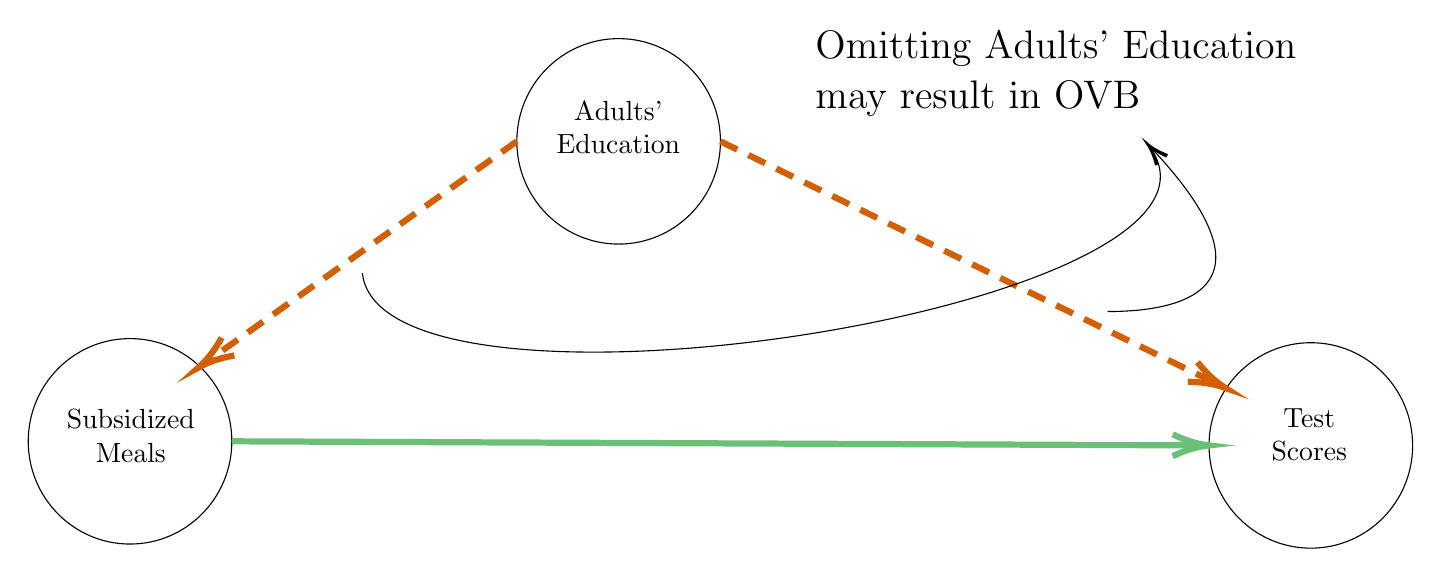
\begin{tikzpicture}[x=0.75pt,y=0.75pt,yscale=-1,xscale=1]
%uncomment if require: \path (0,285); %set diagram left start at 0, and has height of 285

%Shape: Ellipse [id:dp36615011120920427] 
\draw   (254.41,66.5) .. controls (254.41,39.16) and (276.37,17) .. (303.46,17) .. controls (330.54,17) and (352.5,39.16) .. (352.5,66.5) .. controls (352.5,93.83) and (330.54,115.99) .. (303.46,115.99) .. controls (276.37,115.99) and (254.41,93.83) .. (254.41,66.5) -- cycle ;
%Shape: Ellipse [id:dp34906029723118115] 
\draw   (19,211.02) .. controls (19,183.69) and (40.96,161.53) .. (68.04,161.53) .. controls (95.13,161.53) and (117.09,183.69) .. (117.09,211.02) .. controls (117.09,238.36) and (95.13,260.52) .. (68.04,260.52) .. controls (40.96,260.52) and (19,238.36) .. (19,211.02) -- cycle ;
%Shape: Ellipse [id:dp6974919182309072] 
\draw   (587.91,213) .. controls (587.91,185.67) and (609.87,163.51) .. (636.96,163.51) .. controls (664.04,163.51) and (686,185.67) .. (686,213) .. controls (686,240.34) and (664.04,262.5) .. (636.96,262.5) .. controls (609.87,262.5) and (587.91,240.34) .. (587.91,213) -- cycle ;
%Straight Lines [id:da04124970397057681] 
\draw [color={rgb, 255:red, 126; green, 211; blue, 33 }  ,draw opacity=1 ][line width=2.25]    (117.09,211.02) -- (583.91,212.99) ;
\draw [shift={(587.91,213)}, rotate = 180.24] [color={rgb, 255:red, 126; green, 211; blue, 33 }  ,draw opacity=1 ][line width=2.25]    (17.49,-5.26) .. controls (11.12,-2.23) and (5.29,-0.48) .. (0,0) .. controls (5.29,0.48) and (11.12,2.23) .. (17.49,5.26)   ;
%Straight Lines [id:da035209354566531736] 
\draw [color={rgb, 255:red, 255; green, 0; blue, 0 }  ,draw opacity=1 ][line width=2.25]  [dash pattern={on 6.75pt off 4.5pt}]  (254.41,66.5) -- (104.26,173.18) ;
\draw [shift={(101,175.5)}, rotate = 324.6] [color={rgb, 255:red, 255; green, 0; blue, 0 }  ,draw opacity=1 ][line width=2.25]    (17.49,-5.26) .. controls (11.12,-2.23) and (5.29,-0.48) .. (0,0) .. controls (5.29,0.48) and (11.12,2.23) .. (17.49,5.26)   ;
%Straight Lines [id:da19389419961485554] 
\draw [color={rgb, 255:red, 255; green, 0; blue, 0 }  ,draw opacity=1 ][line width=2.25]  [dash pattern={on 6.75pt off 4.5pt}]  (352.5,66.5) -- (592.16,183.53) ;
\draw [shift={(595.76,185.29)}, rotate = 206.03] [color={rgb, 255:red, 255; green, 0; blue, 0 }  ,draw opacity=1 ][line width=2.25]    (17.49,-5.26) .. controls (11.12,-2.23) and (5.29,-0.48) .. (0,0) .. controls (5.29,0.48) and (11.12,2.23) .. (17.49,5.26)   ;
%Curve Lines [id:da92152652585756] 
\draw    (539,148.5) .. controls (571.84,148.5) and (626.45,139.59) .. (559.03,68.58) ;
\draw [shift={(558,67.5)}, rotate = 46.22] [color={rgb, 255:red, 0; green, 0; blue, 0 }  ][line width=0.75]    (10.93,-3.29) .. controls (6.95,-1.4) and (3.31,-0.3) .. (0,0) .. controls (3.31,0.3) and (6.95,1.4) .. (10.93,3.29)   ;
%Curve Lines [id:da6333756929191379] 
\draw    (180,130) .. controls (188.96,212.59) and (617.68,146.17) .. (558.92,68.67) ;
\draw [shift={(558,67.5)}, rotate = 50.63] [color={rgb, 255:red, 0; green, 0; blue, 0 }  ][line width=0.75]    (10.93,-3.29) .. controls (6.95,-1.4) and (3.31,-0.3) .. (0,0) .. controls (3.31,0.3) and (6.95,1.4) .. (10.93,3.29)   ;

% Text Node
\draw (32.08,194.51) node [anchor=north west][inner sep=0.75pt]   [align=left] {\begin{minipage}[lt]{52.62pt}\setlength\topsep{0pt}
\begin{center}
Subsidized\\Meals
\end{center}

\end{minipage}};
% Text Node
\draw (269.97,45.97) node [anchor=north west][inner sep=0.75pt]   [align=left] {\begin{minipage}[lt]{48.09pt}\setlength\topsep{0pt}
\begin{center}
Adults'\\Education
\end{center}

\end{minipage}};
% Text Node
\draw (397,12) node [anchor=north west][inner sep=0.75pt]  [font=\Large] [align=left] {Omitting Adults' Education\\may result in OVB};
% Text Node
\draw (611.97,193.97) node [anchor=north west][inner sep=0.75pt]   [align=left] {\begin{minipage}[lt]{34.47pt}\setlength\topsep{0pt}
\begin{center}
Test\\Scores
\end{center}

\end{minipage}};


\end{tikzpicture}
}
\end{figure}
\end{center}

Again, both conditions must hold for the omission of $Z$ to result in omitted variable bias.

\end{frame}




\begin{frame}{Omitted Variable Bias (OVB)}

There are systematic differences in educational attainment across districts with low and high share of subsidized meals.
\begin{itemize}
    \item Districts more educated adults have higher test scores
    \item Districts less educated adults have more schools with subsidized meals
    \item Among districts with comparable adults' educational attainment, the effect of subsidized meals is generally smaller
\end{itemize}
\begin{center}
        \resizebox{.9\linewidth}{!}{%
            \begin{tabular}{l|cc|cc|cc|}
            \cline{2-7}
                                                                          & \multicolumn{2}{c|}{\begin{tabular}[c]{@{}c@{}}Above-median\\ \% Subsidized meals\end{tabular}} & \multicolumn{2}{c|}{\begin{tabular}[c]{@{}c@{}}Below-median\\ \% Subsidized meals\end{tabular}} & \multicolumn{2}{c|}{\begin{tabular}[c]{@{}c@{}}Difference in\\ Test Scores\end{tabular}} \\ \cline{2-7} 
                                                                          & \multicolumn{1}{c|}{$\overline{Y}$}                            & $n$                            & \multicolumn{1}{c|}{$\overline{Y}$}                            & $n$                            & \multicolumn{1}{c|}{$\overline{Y}^1-\overline{Y}^0$}              & $t$                  \\ \hline
            \multicolumn{1}{|l|}{} &                                                                &                                &                                                                &                                & \multicolumn{1}{c|}{}                                             &                      \\
            \multicolumn{1}{|l|}{\textbf{\textit{All Districts}}}                  & 720.2472                                                       & 250                            & 787.4612                                                       & 250                            & \multicolumn{1}{c|}{67.214}                                       & 15.0000              \\ 
            \multicolumn{1}{|l|}{} &                                                                &                                &                                                                &                                & \multicolumn{1}{c|}{}                                             &                      \\\hline
            \multicolumn{1}{|l|}{} &                                                                &                                &                                                                &                                & \multicolumn{1}{c|}{}                                             &                      \\
            \multicolumn{1}{|l|}{\textbf{\textit{By Share w/ College Education:}}} &                                                                &                                &                                                                &                                & \multicolumn{1}{c|}{}                                             &                      \\
            \multicolumn{1}{|l|}{} &                                                                &                                &                                                                &                                & \multicolumn{1}{c|}{}                                             &                      \\
            \multicolumn{1}{|l|}{{[}0; .1339436{]}}                       & 710.3194                                                       & 108                            & 745.3444                                                       & 18                             & \multicolumn{1}{c|}{35.025}                                       & 2.9064               \\
            \multicolumn{1}{|l|}{{[}.1350751; .1996677{]}}                & 724.0533                                                       & 90                             & 758.4917                                                       & 36                             & \multicolumn{1}{c|}{34.43834}                                     & 4.2446               \\
            \multicolumn{1}{|l|}{{[}.1997542; .3260502{]}}                & 731.9475                                                       & 40                             & 774.4559                                                       & 84                             & \multicolumn{1}{c|}{42.50845}                                     & 5.2279               \\
            \multicolumn{1}{|l|}{{[}.3309678 ; .7696404{]}}               & 742.05                                                         & 12                             & 813.2955                                                       & 112                            & \multicolumn{1}{c|}{71.24553}                                     & 4.2628               \\ \hline
            \end{tabular}
            
}

\end{center}

\end{frame}


\begin{frame}{Identifying Causal Effects}
\begin{itemize}
    \item Here, we are interested in identifying the causal average treatment effect of the share of subsidized meals on test scores (we are not focused on prediction)
    \item Causality implies understanding if changes in one variable \textbf{cause} changes in another \textbf{irrespective} of all other factors.
    \item To achieve this goal, we want to make \textbf{ceteris paribus} comparisons
    \item It is often useful to think of a causal effect as the one measured in an ideal \textbf{randomized controlled experiment (RCT)}.
    \begin{itemize}
        %\item \textit{Ideal}: subjects all follow the treatment protocol – perfect compliance, no errors in reporting, etc.
        \item \textit{Randomized}: subjects from the population of interest are randomly assigned to a treatment or control group (so there are no confounding factors)
        \item \textit{Controlled}: having a control group permits measuring the differential effect of the treatment
        \item \textit{Experiment}: the treatment is assigned as part of the experiment: the subjects have no choice, so there is no “reverse causality” in which subjects choose the treatment they think will work best.
    \end{itemize}
    \item In an ideal RCT, meal subsidies would be randomly allocated to schools, i.e., irrespective of any pre-existing differences across school districts.
\end{itemize}
\end{frame}



\begin{frame}{Identifying Causal Effects}

Clearly, this is not the case here: treatment and control groups differ in systematic ways.

\begin{center}
        \resizebox{.9\linewidth}{!}{%
            \begin{tabular}{l|cc|cc|cc|}
            \cline{2-7}
                                                                          & \multicolumn{2}{c|}{\begin{tabular}[c]{@{}c@{}}Above-median\\ \% Subsidized meals\end{tabular}} & \multicolumn{2}{c|}{\begin{tabular}[c]{@{}c@{}}Below-median\\ \% Subsidized meals\end{tabular}} & \multicolumn{2}{c|}{\begin{tabular}[c]{@{}c@{}}Difference in\\ Test Scores\end{tabular}} \\ \cline{2-7} 
                                                                          & \multicolumn{1}{c|}{$\overline{Y}$}                            & $n$                            & \multicolumn{1}{c|}{$\overline{Y}$}                            & $n$                            & \multicolumn{1}{c|}{$\overline{Y}^1-\overline{Y}^0$}              & $t$                  \\ \hline
            \multicolumn{1}{|l|}{} &                                                                &                                &                                                                &                                & \multicolumn{1}{c|}{}                                             &                      \\
            \multicolumn{1}{|l|}{\textbf{\textit{All Districts}}}                  & 720.2472                                                       & 250                            & 787.4612                                                       & 250                            & \multicolumn{1}{c|}{67.214}                                       & 15.0000              \\ 
            \multicolumn{1}{|l|}{} &                                                                &                                &                                                                &                                & \multicolumn{1}{c|}{}                                             &                      \\\hline
            \multicolumn{1}{|l|}{} &                                                                &                                &                                                                &                                & \multicolumn{1}{c|}{}                                             &                      \\
            \multicolumn{1}{|l|}{\textbf{\textit{By Share w/ College Education:}}} &                                                                &                                &                                                                &                                & \multicolumn{1}{c|}{}                                             &                      \\
            \multicolumn{1}{|l|}{} &                                                                &                                &                                                                &                                & \multicolumn{1}{c|}{}                                             &                      \\
            \multicolumn{1}{|l|}{{[}0; .1339436{]}}                       & 710.3194                                                       & 108                            & 745.3444                                                       & 18                             & \multicolumn{1}{c|}{35.025}                                       & 2.9064               \\
            \multicolumn{1}{|l|}{{[}.1350751; .1996677{]}}                & 724.0533                                                       & 90                             & 758.4917                                                       & 36                             & \multicolumn{1}{c|}{34.43834}                                     & 4.2446               \\
            \multicolumn{1}{|l|}{{[}.1997542; .3260502{]}}                & 731.9475                                                       & 40                             & 774.4559                                                       & 84                             & \multicolumn{1}{c|}{42.50845}                                     & 5.2279               \\
            \multicolumn{1}{|l|}{{[}.3309678 ; .7696404{]}}               & 742.05                                                         & 12                             & 813.2955                                                       & 112                            & \multicolumn{1}{c|}{71.24553}                                     & 4.2628               \\ \hline
            \end{tabular}
            
}

\end{center}

\end{frame}

\begin{frame}{Another way to see this}
\begin{center}
    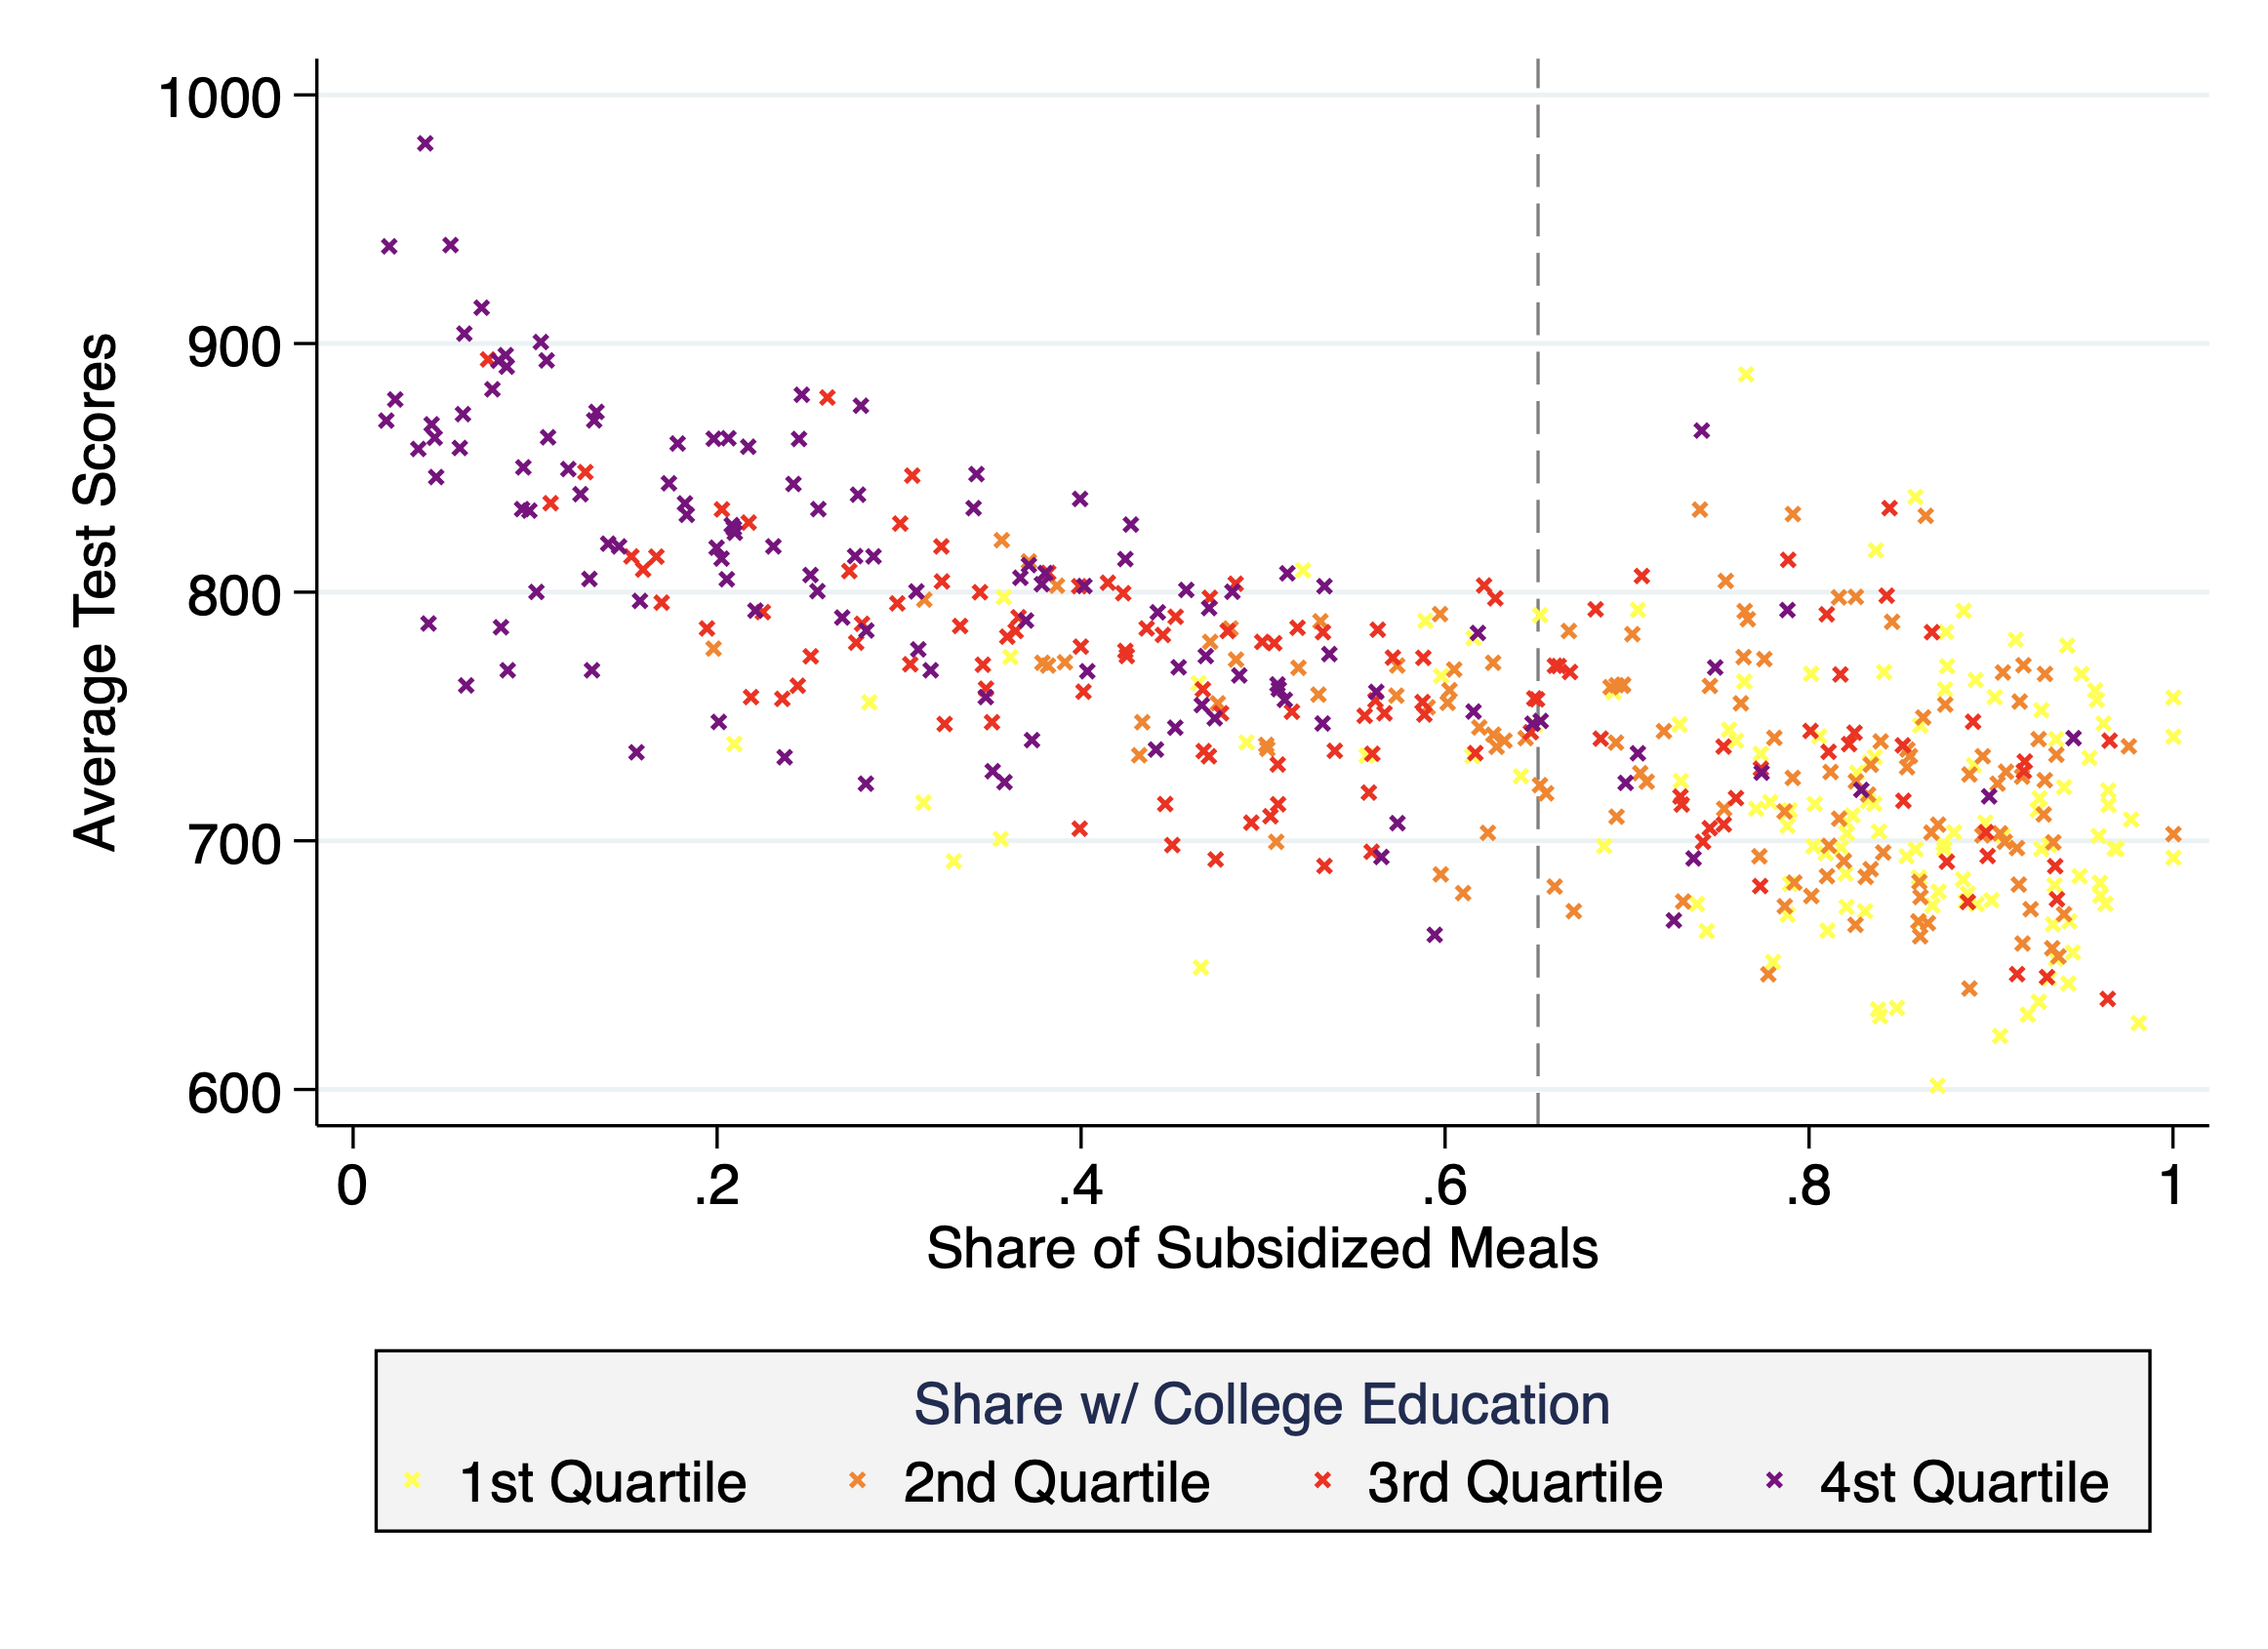
\includegraphics[scale=.27]{images/testscores_group5.png}
\end{center}

\end{frame}

\begin{frame}{Another way to see this}
\begin{center}
    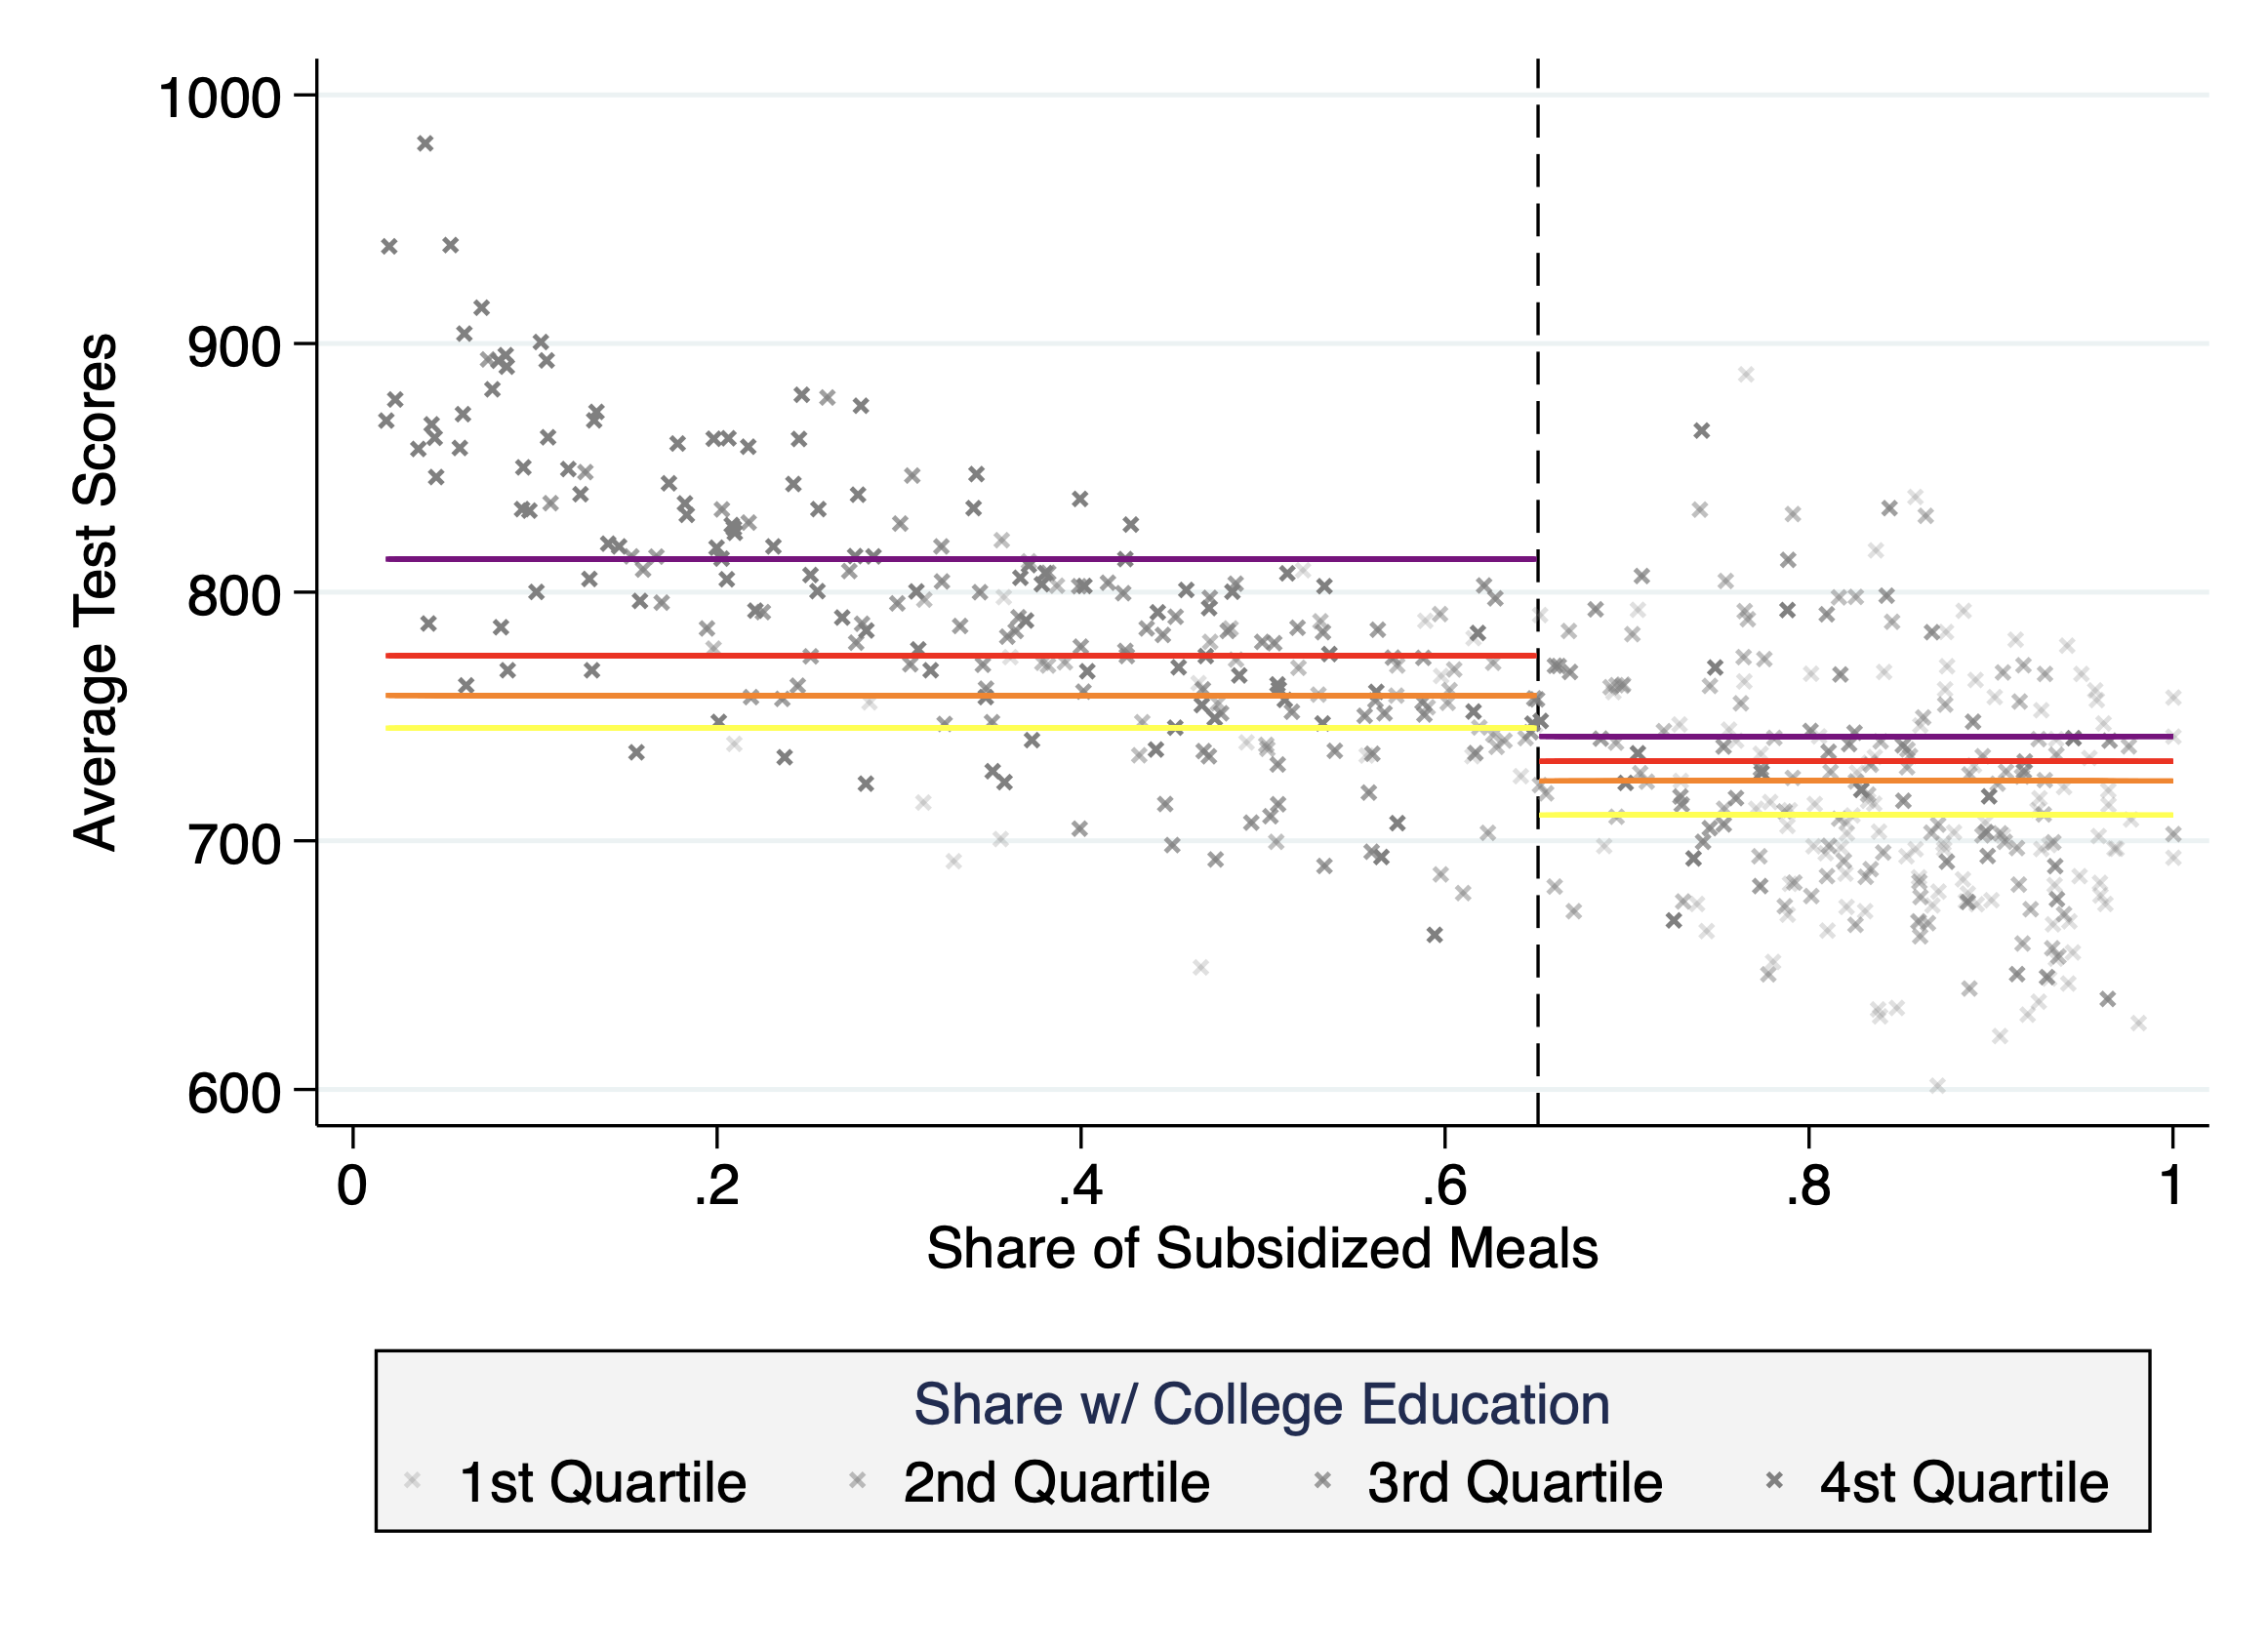
\includegraphics[scale=.27]{images/testscores_group6.png}
\end{center}

\end{frame}


\begin{frame}{What to do about it?}
\begin{itemize}
    \item Randomization implies that any differences between the treatment and control groups are random --- not systematically related to the treatment
    \item From now on, one of the main goals of this course is to explore ways to recover causal treatment effects
    \item Remember, we want to make ceteris paribus, apple-to-apple comparisons --- not pear-to-apple, etc.
    \item One way to do it is to \textbf{control} for systematic differences between control and treatment group
    \item In our example, we want to know the average treatment effect of subsidizing school meals on test scores, holding the share of college education, average income, English proficiency, etc. constant (i.e., getting closer to all else equal, or ceteris paribus)
    \item Said differently, we want to know the average impact of a change in subsidized meals on test scores within groups where college education, average income, English proficiency, etc. is the same
\end{itemize}

\end{frame}


\begin{frame}{The Multiple Regression Model }
\begin{equation*}
    Y_i = \beta_{0} + \beta_1 X_{1i} + \beta_2 X_{2i} + ... + \beta_k X_{ki} + u_i \text{~~~~~~with~~} i=1,\dots, n
\end{equation*}
Where
\begin{itemize}
    \item $Y_i$ is the $i$th observation of the dependant variable
    \item $X_{1i}, X_{2i}, ..., X_{ki}$ is the $i$th observation of the $k$th regressor
    \item $u_i$ is the error term
\end{itemize}
\vspace{.5cm}
The population regression line is therefore given by:
\begin{equation*}
     \mathbb{E}(Y_i\mid X_{1i}=x_1, X_{2i}=x_2, ..., X_{ki}=x_k) = \beta_0 + \beta_1 x_1 + \beta_2 x_2 + ... + \beta_k x_k 
\end{equation*}
\begin{itemize}
    \item $\beta_k$ is the slope of $X_{ki}$
    \item $\beta_k$ is the expected difference in $Y_i$ associated with a unit change in $X_{ki}$ holding all other regressors constant
    \item $\beta_0$, the intercept, can be thought of as the coefficient on a regressor $X_{0i}$ that is equal to 1 for all observations. $\beta_0$ is the expected value of $Y_i$ when all $X_{ki}$ are equal to zero.
\end{itemize}

\end{frame}


\begin{frame}{Example for $k=2$}
Imagine we compare two schools, $i$ and $j$
\begin{eqnarray*}
\begin{cases}
    Y_i = \beta_{0} + \beta_1 X_{1i} + \beta_2 X_{2i}\\
    Y_j = \beta_{0} + \beta_1 X_{1j} + \beta_2 X_{2j}\\
\end{cases}\\
\Rightarrow
\begin{cases}
    Y_i = \beta_{0} + \beta_1 X_{1i} + \beta_2 X_{2i}\\
    Y_i + \Delta Y_i = \beta_{0} + \beta_1 (X_{1i}+ \Delta X_{1i}) + \beta_2 (X_{2j} + \Delta X_{2i})\\
\end{cases}\\
\Rightarrow
\Delta Y_i = \beta_1 \Delta X_{1i} + \beta_2 \Delta X_{2i}
\end{eqnarray*}
When $X_2$ is constant, i.e., $X_{2i}=X_{2j}$, then $\Delta X_{2i}=0$ and therefore,
\begin{equation*}
    \Delta Y_i = \beta_1 \Delta X_{1i}
\end{equation*}
In general, holding all other regressors constant, $\frac{\Delta Y_i}{\Delta X_{1i}}= \beta_1$.
\end{frame}


\begin{frame}{The OLS Estimator in Multiple Regression}
As with simple regression, OLS estimators $\hat{\beta}_0, \hat{\beta}_1, \hat{\beta}_2, ... , \hat{\beta}_k$ solve

\begin{equation*}
    \min_{b_0, b_1, b_2, ..., b_k} \sum_{i=1}^n (Y_i - b_0 - b_1 X_{1i}- b_2 X_{2i}-...- b_k X_{ki})^2
\end{equation*}
The derivative of the sum of squared prediction mistakes with respect to the $j$th regression coefficient, $b_j$, is
\begin{eqnarray*}
    \frac{\partial}{\partial b_j} = \sum_{i=1}^n (Y_i - b_0 - b_1 X_{1i}- b_2 X_{2i}-...- b_k X_{ki})^2\\
    \Leftrightarrow -2 \sum_{i=1}^n X_{ji} (Y_i - b_0 - b_1 X_{1i}- b_2 X_{2i}-...- b_k X_{ki})
\end{eqnarray*}
Combined, these yield the system of $k+1$ equations that, when set to 0, constitute the first-order conditions for the OLS estimator, $\bm{\hat{\beta}}$ --- the $(k+1)\times1$ dimensional vector of the $k+1$ estimates of the unknown regression coefficients

\end{frame}


\begin{frame}{The OLS Estimator in Multiple Regression}
The system of equation can be written as (with matricial notation)
\begin{eqnarray*}
    \bm{-2_{k+1}X'(Y-X\hat{\beta})=0_{k+1}}\\
    \Rightarrow \bm{X'Y-X'X\hat{\beta}=0_{k+1}}\\
    \Rightarrow \bm{\hat{\beta}=(X'X)^{-1}X'Y}\\
\end{eqnarray*}
Where
\begin{eqnarray*}
    \bm{Y}_{n\times1}=\begin{bmatrix}
Y_1\\
Y_2\\
.\\
.\\
.\\
Y_n
\end{bmatrix}
\text{~;~~~~~}   \bm{X}_{n\times (k+1)}=\begin{bmatrix}
1 & X_{11} & X_{21} & \dots & X_{k1}\\
1 & X_{12} & X_{22} & \dots & X_{k2}\\
. & . & . & \dots & .\\
. & . & . & \dots & .\\
. & . & . & \dots & .\\
1 & X_{1n} & X_{2n} & \dots & X_{kn}\\
\end{bmatrix}
\text{~;~and~~~} \bm{\hat{\beta}}_{(k+1)\times1}=\begin{bmatrix}
\hat{\beta}_0\\
\hat{\beta}_1\\
.\\
.\\
.\\
\hat{\beta}_k
\end{bmatrix}
\end{eqnarray*}
\end{frame}


\begin{frame}{Example: The impact of Subsidized Meals on Test Scores }
\begin{center}
    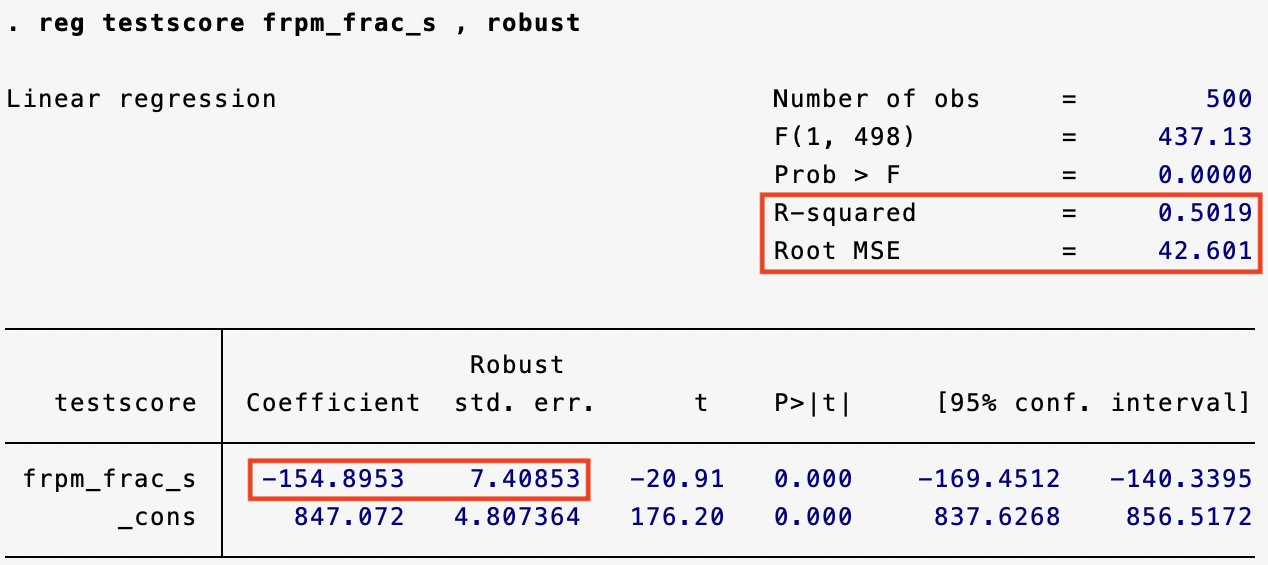
\includegraphics[scale=.6]{images/regcontr0.png}
\end{center}
\end{frame}

\begin{frame}{Example: The impact of Subsidized Meals on Test Scores }
\begin{center}
    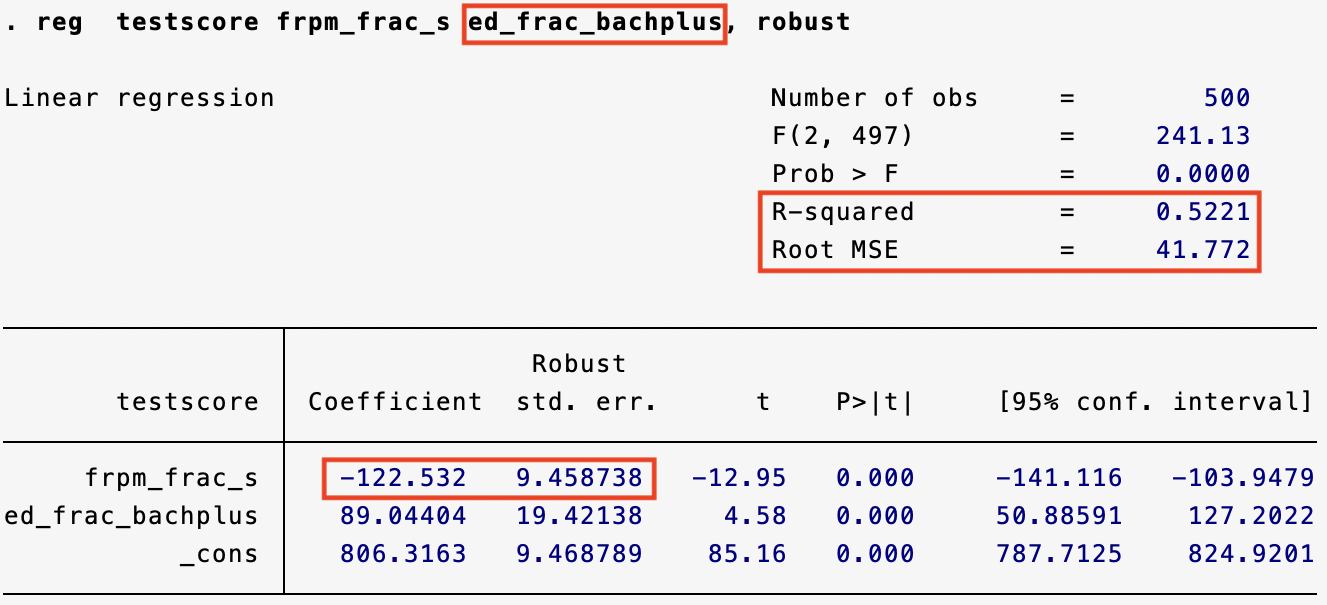
\includegraphics[scale=.6]{images/regcontr1.png}
\end{center}
\end{frame}


\begin{frame}{Goodness of Fit in Multiple Regression}
Remember that:
\begin{center}
    Actual = Predicted + Residual ($Y_i= \hat{Y}_i+\hat{u}_i$)
\end{center}
In the previous lectures, we have seen that:

\begin{itemize}
    \item RMSE = std. deviation of $\hat{u}_i$ \textit{without} d.f. correction
    \item SER = std. deviation of $\hat{u}_i$ \textit{with} d.f. correction
    \item $R^2$ = share of the variance of $Y$ explained by $X$ \textit{without} d.f. correction
\end{itemize}
Now, we will introduced the adjusted $R^2$, written $\overline{R}^2$
\begin{itemize}
    \item[$\Rightarrow$] $\overline{R}^2$ = share of the variance of $Y$ explained by $X$ \textit{with} d.f. correction
\end{itemize}
\end{frame}

\begin{frame}{Goodness of Fit in Multiple Regression}
With multiple regressors,
\begin{itemize}
    \item RMSE = $\sqrt{\frac{1}{n}\sum_{i=1}^n \hat{u}_i^2}$
    \item SER = $\sqrt{\frac{1}{n-(k+1)}\sum_{i=1}^n \hat{u}_i^2}$
    \item $R^2$ = $\frac{\sum_{i=1}^n(\hat{Y}_i-\overline{{Y}})^2}{\sum_{i=1}^n({Y}_i-\overline{Y})^2}= 1-\frac{\sum_{i=1}^n \hat{u}_i^2}{\sum_{i=1}^n({Y}_i-\overline{Y})^2}$
\end{itemize}
\vspace{1cm}
BUT whenever a variable is added to the RHS, the sum of squared residuals is (almost systematically) smaller (the OLS finds the values of the coefficients that minimize
the sum of squared residuals) so the $SSR \downarrow\Rightarrow R^2 \uparrow$
\end{frame}

\begin{frame}{Goodness of Fit in Multiple Regression}
The $\overline{R}^2$,  ``adjusted'' $R^2$ corrects this by penalizing the inclusion of an additional regressor:
\begin{equation*}
    \overline{R}^2 = 1- \frac{n-1}{n-k-1}\frac{\sum_{i=1}^n \hat{u}_i^2}{\sum_{i=1}^n(\hat{Y}_i-\overline{Y})^2}
\end{equation*}
Note that:
\begin{itemize}
    \item $\overline{R}^2<R^2$ because $\frac{n-1}{n-k-1}>1$ but when $n\rightarrow\infty$ they become very close.
    \item Adding one regressor $\downarrow SSR$ but also $\uparrow\frac{n-1}{n-k-1}$
    \item $\overline{R}^2$ may be negative if the (many) regressors $\downarrow SSR$ but $\uparrow\uparrow\uparrow\frac{n-1}{n-k-1}$
\end{itemize}
\vspace{.5cm}
However, including a variable in a multiple regression should be based on whether including that variable allows you to better identify the causal effect of interest.
\end{frame}

\begin{frame}{The OLS Assumptions for Causal Inference
in the Multiple Regression Model}
\begin{equation*}
    Y_i = \beta_{0} + \beta_1 X_{1i} + \beta_2 X_{2i} + ... + \beta_k X_{ki} + u_i \text{~~~~~~with~~} i=1,\dots, n
\end{equation*}\\
\vspace{.5cm}
where $\beta_1, \dots, \beta_k$ are causal effects and\vspace{.5cm}

\begin{enumerate}
    \item $u_i$ has a conditional mean of 0 given $X_{1i}, X_{2i}, \dots, X_{ki}$; that is,
    \begin{equation*}
        \mathbb{E}(u_i \mid X_{1i}, X_{2i}, \dots, X_{ki})=0
    \end{equation*}
    \item $(X_{1i}, X_{2i}, \dots, X_{ki}, Y_i)$ are i.i.d. draws from their joint distribution.
    \item Large outliers are unlikely: $(X_{1i}, X_{2i}, \dots, X_{ki}, Y_i)$ have nonzero finite fourth moments
    \item There is no perfect multicollinearity.
\end{enumerate}
\vspace{.5cm}
$\Rightarrow$ If assumptions 1-4 hold, then in large samples the OLS estimators $\hat{\beta}_0, \hat{\beta}_1, \dots, \hat{\beta}_k$ are jointly normally distributed, and each $\hat{\beta}_j\sim \mathcal{N}(\beta_j; \sigma^2_{\hat{\beta}_j})$.
\end{frame}


\begin{frame}{What is Multicollinearity?}
 Multicollinearity refers to the high correlation between two or more independent variables in a regression model.\\[1em]
  \begin{itemize}
    \item \textbf{Perfect Multicollinearity:} A linear relationship exists between independent variables (e.g., $X_3 =0.5 \times  \text{Share w/ College Education}$).\\[1em]
    \item \textbf{High Multicollinearity:} High correlation but not a perfect linear relationship (e.g., $\rho(\text{Share w/ College Education; Median Income})=0.8755$).\\[1em]
  \end{itemize}
\end{frame}



\begin{frame}{Example: Perfect Multicolinearity}
\begin{center}
    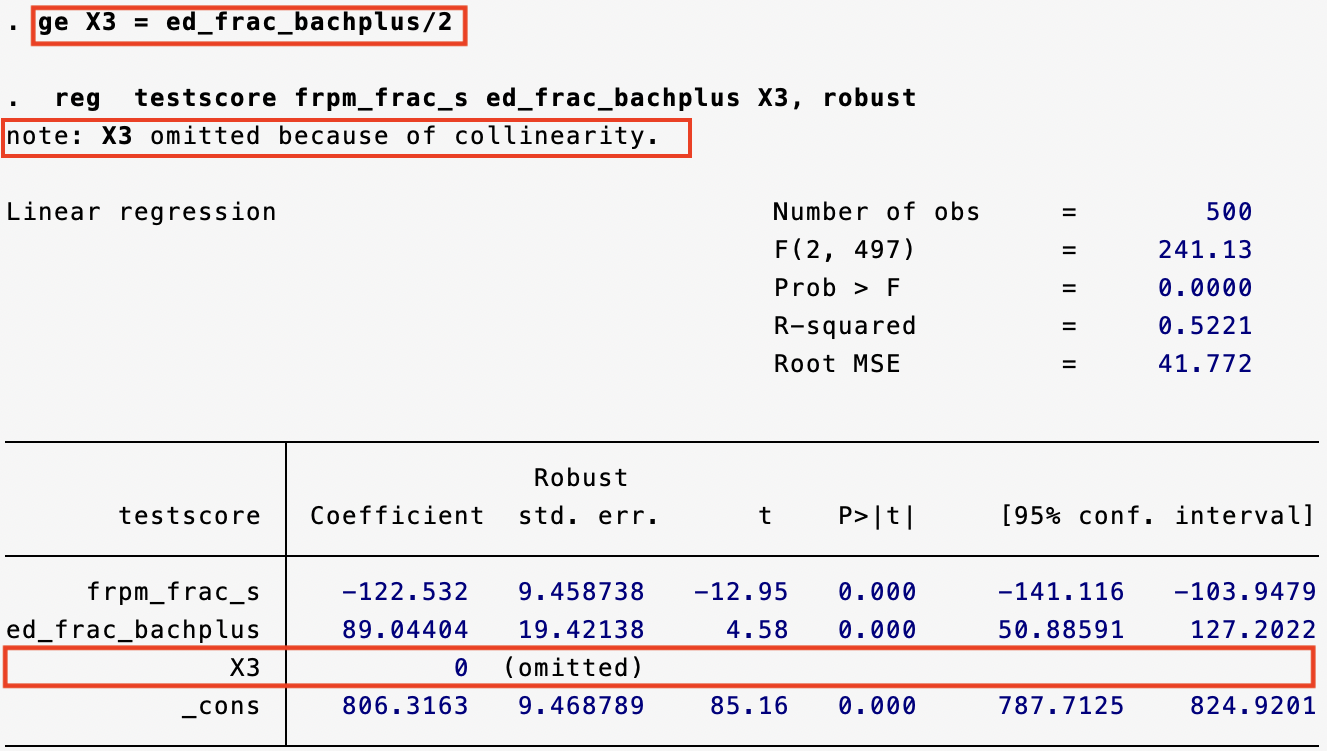
\includegraphics[scale=.56]{images/multicolinearity0.png}
\end{center}
\end{frame}

\begin{frame}{Example: High Multicolinearity}
\begin{center}
    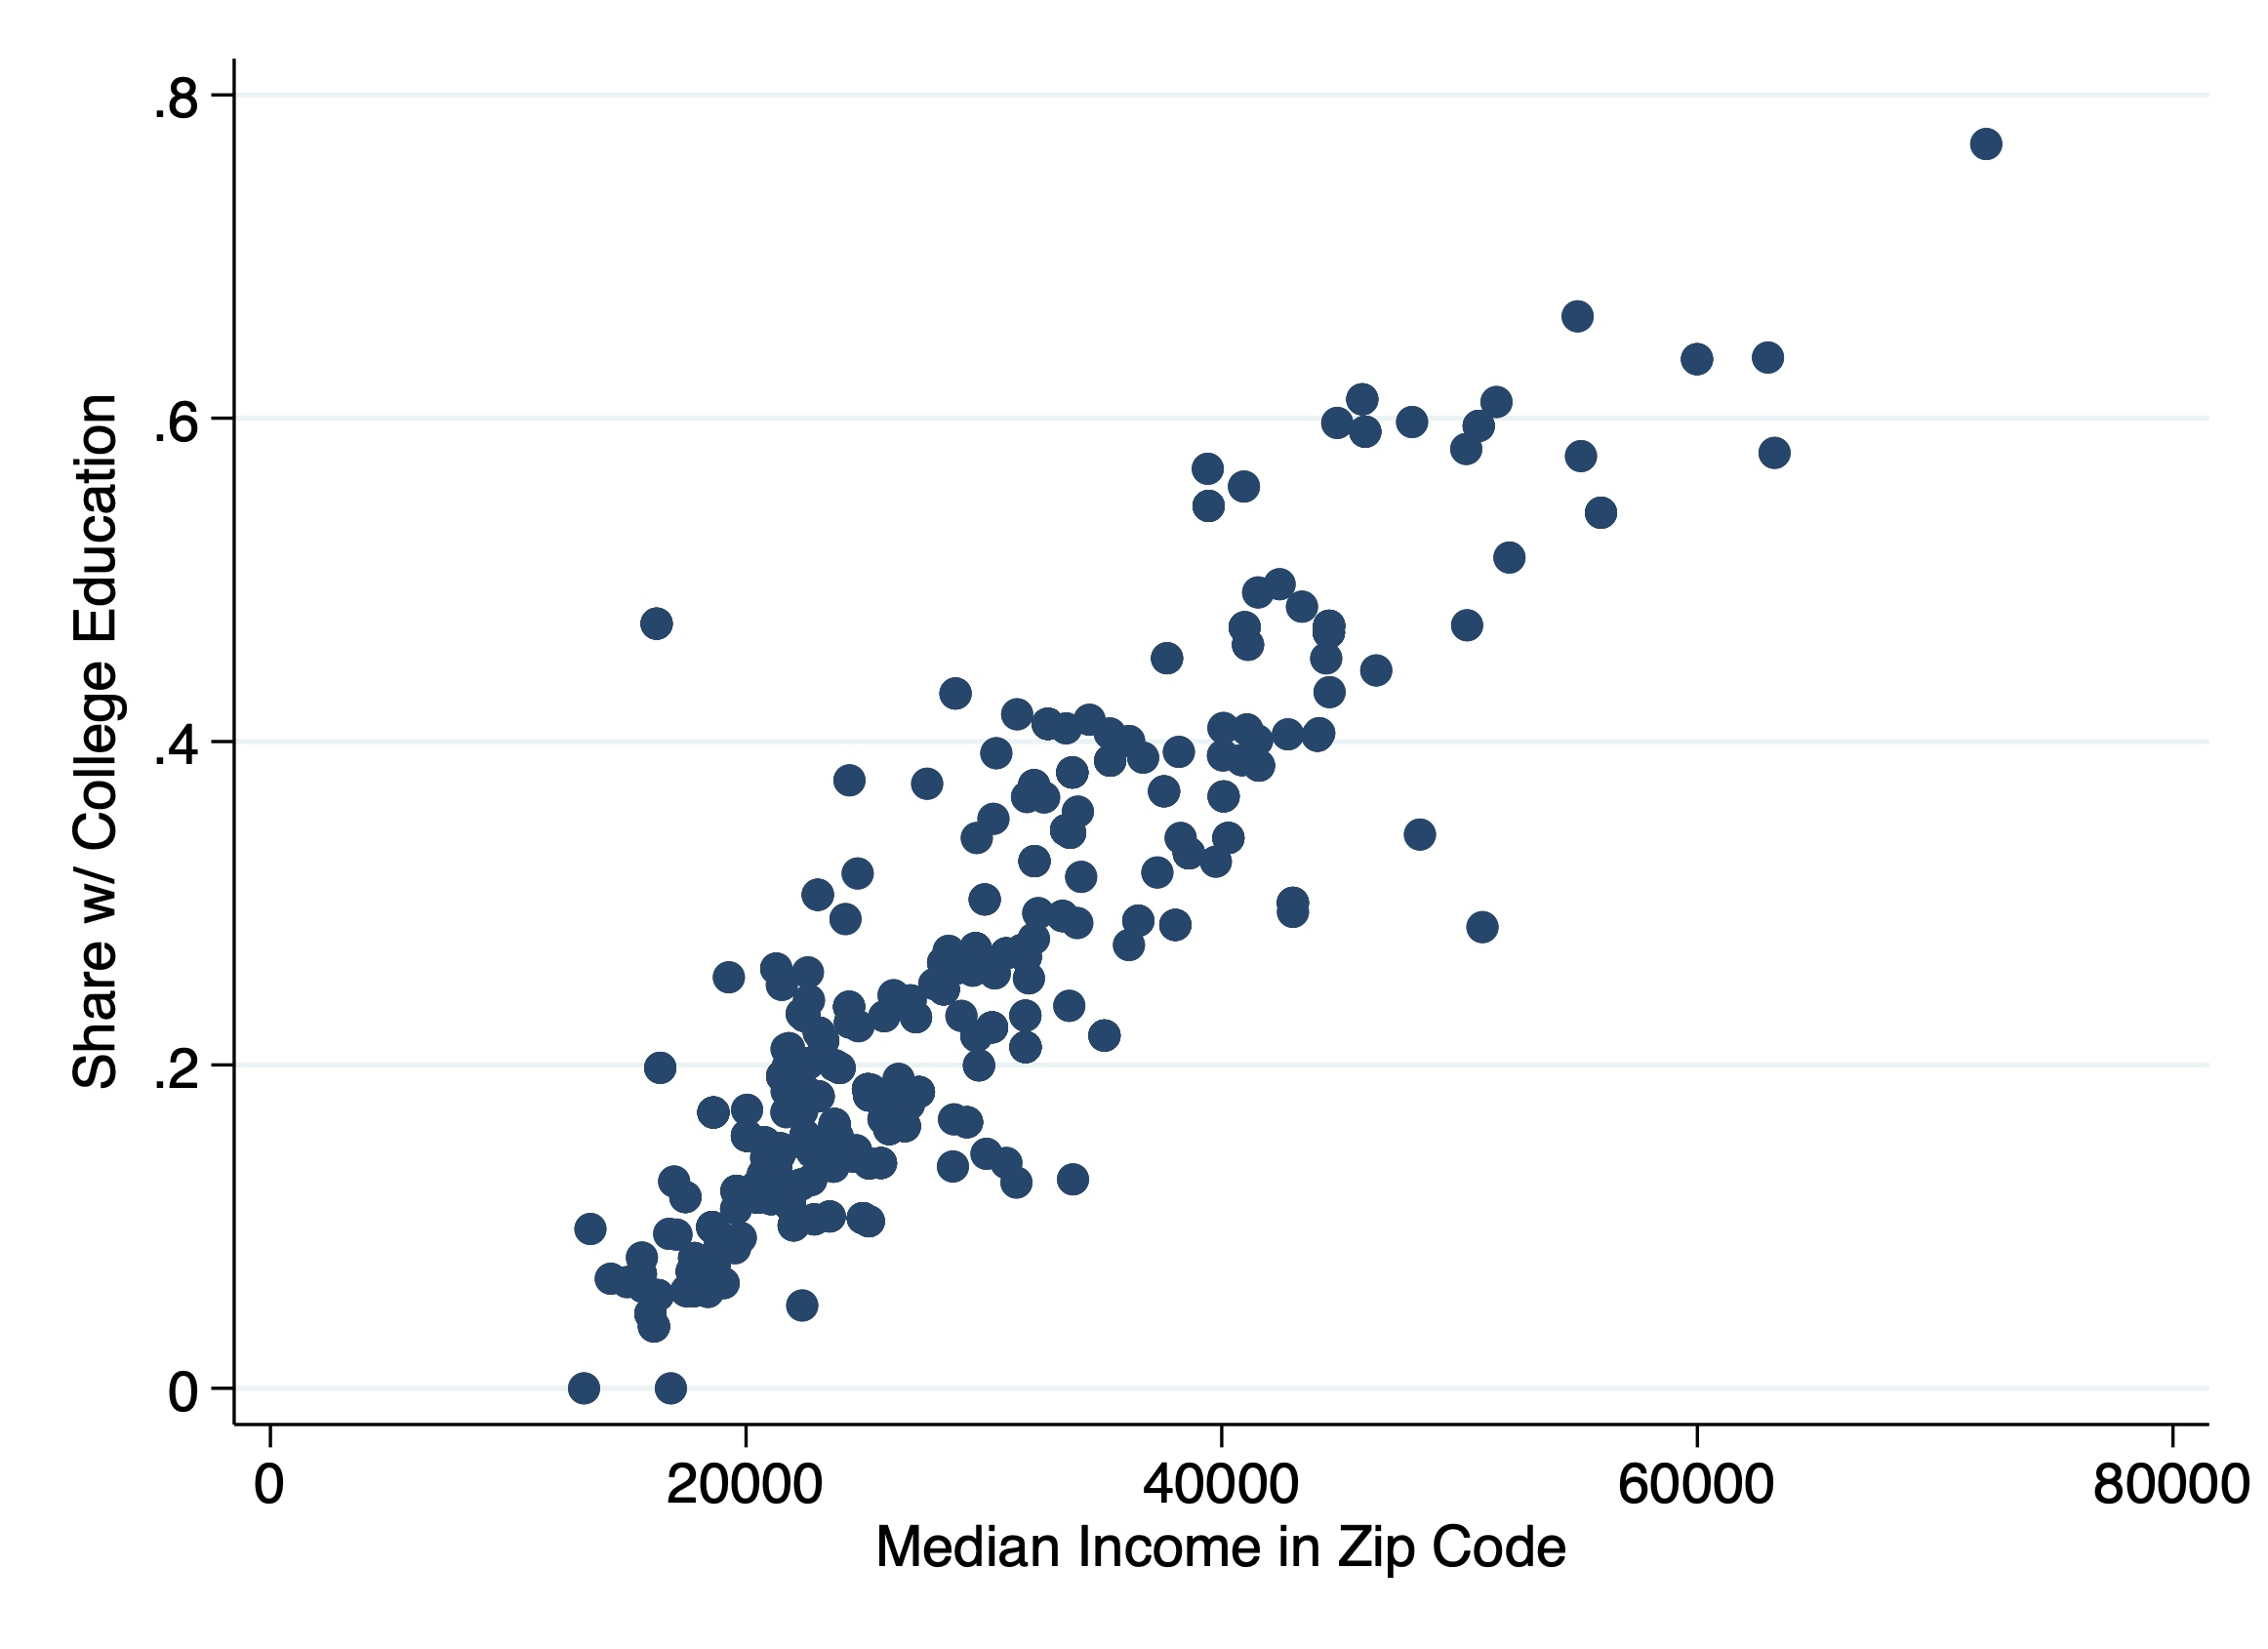
\includegraphics[scale=.13]{images/multicollinearity_illustration.jpg}
\end{center}
\end{frame}

\begin{frame}{Example: High Multicolinearity}
\begin{center}
    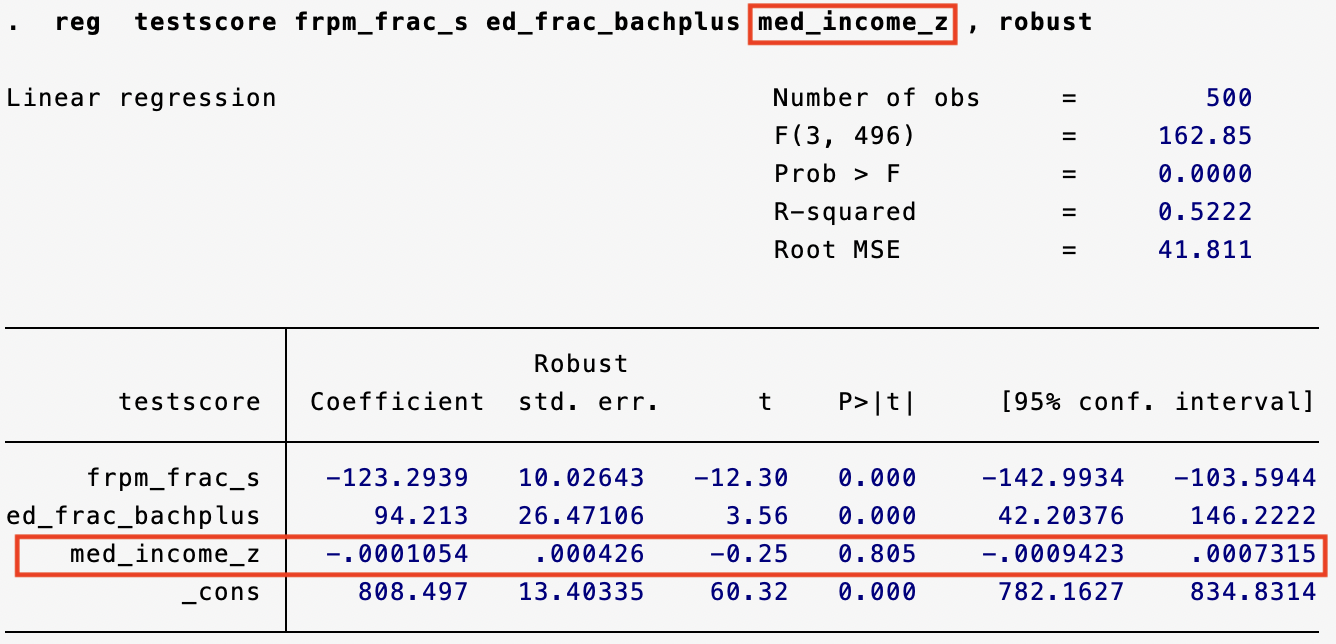
\includegraphics[scale=.6]{images/multicolinearity1.png}
\end{center}
\end{frame}


\begin{frame}{The dummy variable trap}
Suppose you have a set of multiple mutually exclusive and exhaustive variables  --- that is, there are multiple categories and every observation falls in one and only one category (Freshmen, Sophomores, Juniors, Seniors, Other).\\ \vspace{.5cm}

If you include all these variables and a constant (in general, the intercept), you will have perfect multicollinearity --- this is sometimes called the dummy variable trap (as it often occurs with dummy variables).\\ \vspace{.5cm}

We can then decide to omit one of the groups (or the constant). In this case, the coefficients on the included binary variables represent the incremental effect of being in that category, relative to the base case of the omitted category.

\end{frame}

\begin{frame}{Example: Omitted category 1/2}
\begin{center}
    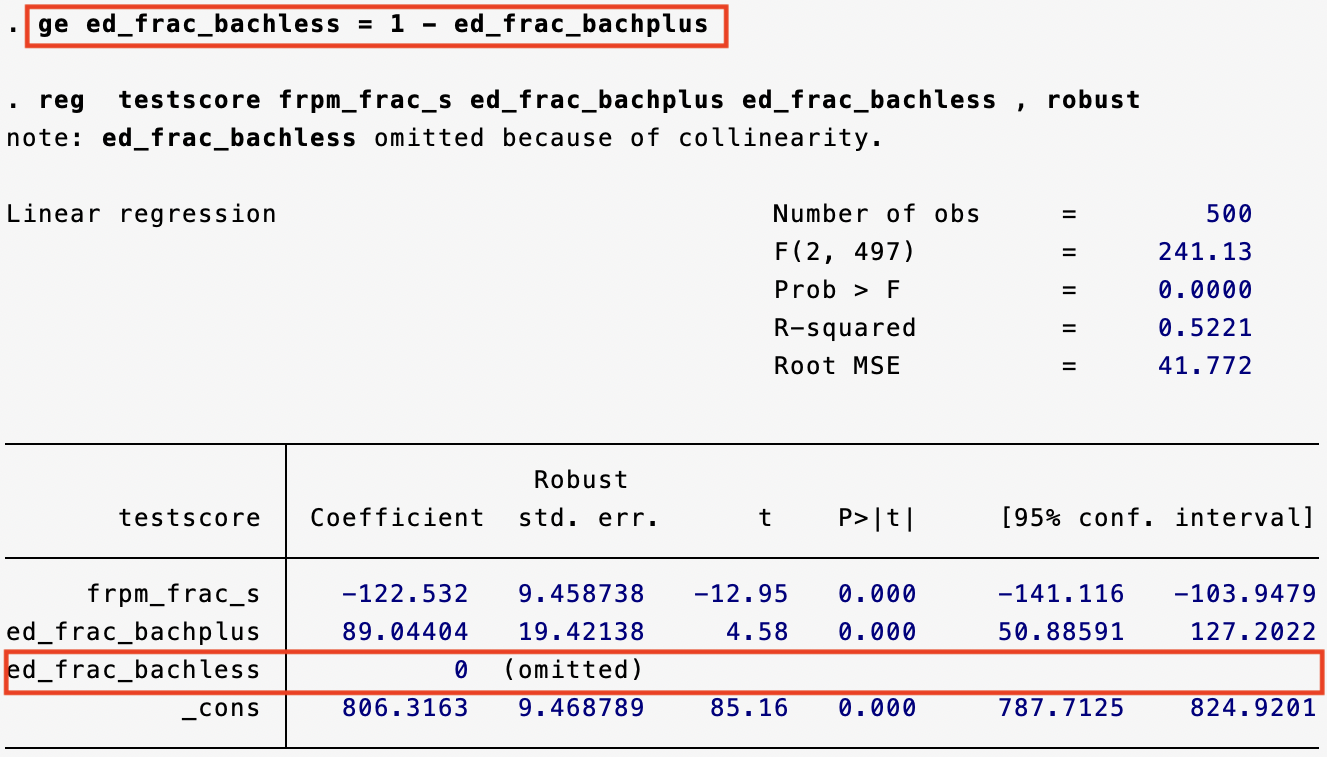
\includegraphics[scale=.56]{images/multicolinearity2.png}
\end{center}
\end{frame}

\begin{frame}{Example: Omitted category 2/2}
\begin{center}
    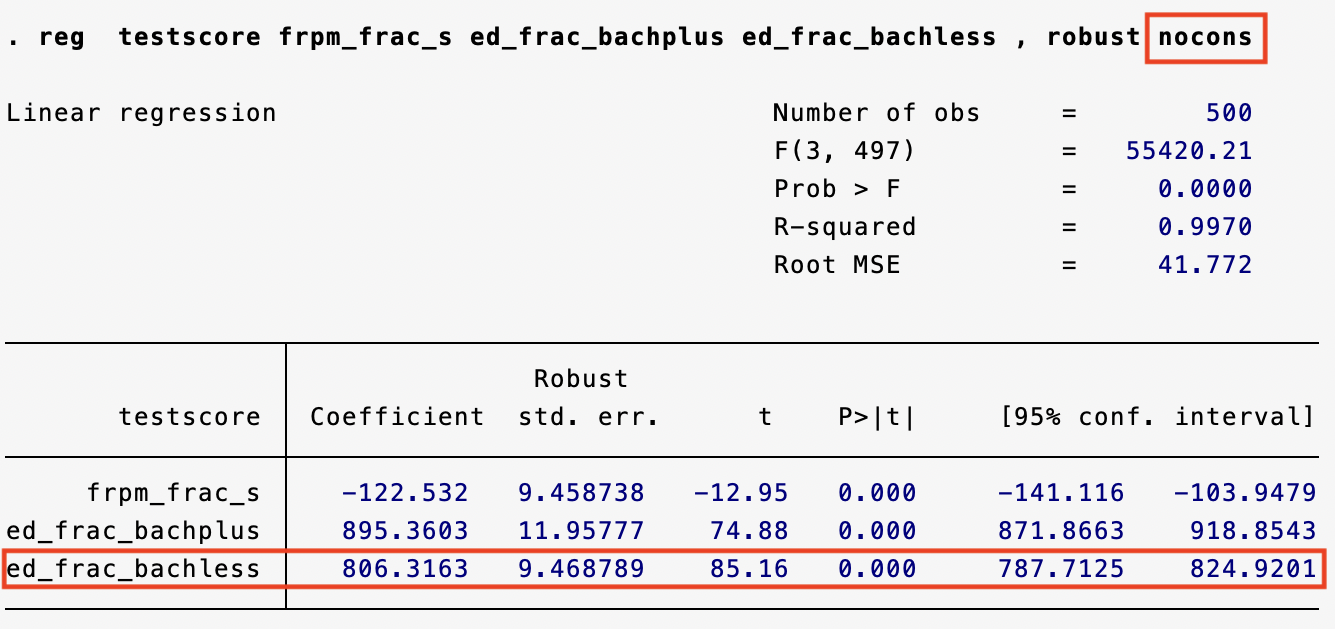
\includegraphics[scale=.6]{images/multicolinearity3.png}
\end{center}
\end{frame}


\begin{frame}{Control Variables in Multivariate Analysis}
    \begin{exampleblock}{Definition}
        A control variable $W$ is a regressor included to hold constant factors that, if neglected, could lead the estimated causal effect of interest to suffer from omitted variable bias.
    \end{exampleblock}

\vspace{.5cm}    This definition means that

    \begin{enumerate}
        \item We need to modify the OLS assumptions such that the OLS estimator of the effect of interest is unbiased, but the OLS coefficients on control variables are, in general, biased and do not have a causal interpretation.
        \item A good control variable is one which, when included in the regression, makes the error term uncorrelated with the variable of interest.
        \item Holding constant the control variable(s), the variable of interest is ``as if'' randomly assigned.
        \item Among individuals (entities) with the same value of the control variable(s), the variable of interest is uncorrelated with the omitted determinants of $Y$
    \end{enumerate}
\end{frame}


\begin{frame}{Conditional Mean Independance}
\begin{itemize}
    \item Because a control variable is correlated with an omitted causal factor, the first OLS Assumption, $\mathbb{E}(u_i \mid X_{1i}, X_{2i}, \dots, X_{ki})=0$ does not hold anymore
    \item We need a mathematical condition for what makes an effective control variable. This condition is the \textit{conditional mean independence}
    \item Given the control variable, the mean of $u_i$ does not depend on the variable of interest
    \item Question: Conditional on sharing the same exposure to adults' educational attainment, is the share of subsidized meals as good as random?
    
\end{itemize}

\end{frame}


\begin{frame}{The OLS Assumptions for Causal Inference
in the Multiple Regression Model with Control Variables}
\begin{equation*}
    Y_i = \beta_{0} + \beta_1 X_{1i} + \beta_2 X_{2i} + ... + \beta_k X_{ki} + \beta_{k+1} W_{1i} + \beta_{k+2} W_{2i} + ... + \beta_{k+r} W_{ri} + u_i \text{~~~~~~with~~} i=1,\dots, n
\end{equation*}\\
\vspace{.5cm}
where $\beta_1, \dots, \beta_k$ are causal effects,  $W_{ji}$ are control variables, and\vspace{.5cm}

\begin{enumerate}
    \item $u_i$ has a conditional mean that does not depend on the $X$’s given the $W$’s; that is,
    \begin{equation*}
        \mathbb{E}(u_i \mid X_{1i}, X_{2i}, \dots, X_{ki},  W_{1i},  W_{2i}, \dots,  W_{ri})=\mathbb{E}(u_i \mid W_{1i},  W_{2i}, \dots,  W_{ri})
    \end{equation*}
    \item $(X_{1i}, X_{2i}, \dots, X_{ki},  W_{1i},  W_{2i}, \dots,  W_{ri}, Y_i)$ are i.i.d. draws from their joint distribution.
    \item Large outliers are unlikely: $(X_{1i}, X_{2i}, \dots, X_{ki},  W_{1i},  W_{2i}, \dots,  W_{ri}, Y_i)$ have nonzero finite fourth moments
    \item There is no perfect multicollinearity.
\end{enumerate}
\vspace{.3cm}
$\Rightarrow$ If assumptions 1-4 hold, then in large samples the OLS estimators of interest, $\hat{\beta}_0, \hat{\beta}_1, \dots, \hat{\beta}_k$ are jointly normally distributed, and each $\hat{\beta}_j\sim \mathcal{N}(\beta_j; \sigma^2_{\hat{\beta}_j})$ BUT $\hat{\beta}_{k+1}, \hat{\beta}_{k+2}, \dots, \hat{\beta}_{k+r}$ might be biased!
\end{frame}



\begin{frame}[allowframebreaks]{Material}
\begin{itemize}
    \item[--] \textbf{Textbooks:}
    \begin{itemize}
        \item Introduction to Econometrics, 4th Edition, Global Edition, by Stock and Watson -- Chapter 6.
    \end{itemize}
\end{itemize}
\end{frame}


\end{document}
